% Appendix E: AgiBot Evaluation Table - In-domain & Unseen
% Fixed multirow syntax and positioning

We provide the evaluation setup for both seen tasks in Tables~\ref{tab:seen_tasks} and unseen tasks in  Table~\ref{tab:unseen_tasks} for Agibot. Each row shows the initial frame and instruction for 4 robots. We conduct 2 rollouts per robot for each task by varying the objects, locations and the robot arm to use for the task (The current table mostly shows the evaluation using the left arm).

% \subsection{Seen Tasks (In-Domain)}

\begin{table*}[htbp]
\centering
\caption{\textbf{Seen Tasks Evaluation Setup for AgiBot G1}}
\label{tab:seen_tasks}
\setlength{\tabcolsep}{2pt}
\resizebox{\textwidth}{!}{
\begin{tabular}{m{1.8cm}cm{1.8cm}m{3.2cm}m{3.2cm}m{3.2cm}m{3.2cm}m{3.2cm}m{3.2cm}m{3.2cm}m{3.2cm}}
\toprule
\centering\textbf{Category} & \centering\textbf{\#} & \centering\textbf{Task} & \centering\textbf{Image} & \centering\textbf{Instruction} & \centering\textbf{Image} & \centering\textbf{Instruction} & \centering\textbf{Image} & \centering\textbf{Instruction} & \centering\textbf{Image} & \centering\arraybackslash\textbf{Instruction} \\
\midrule
 & 1 & \centering\textbf{PnP Fruit} & 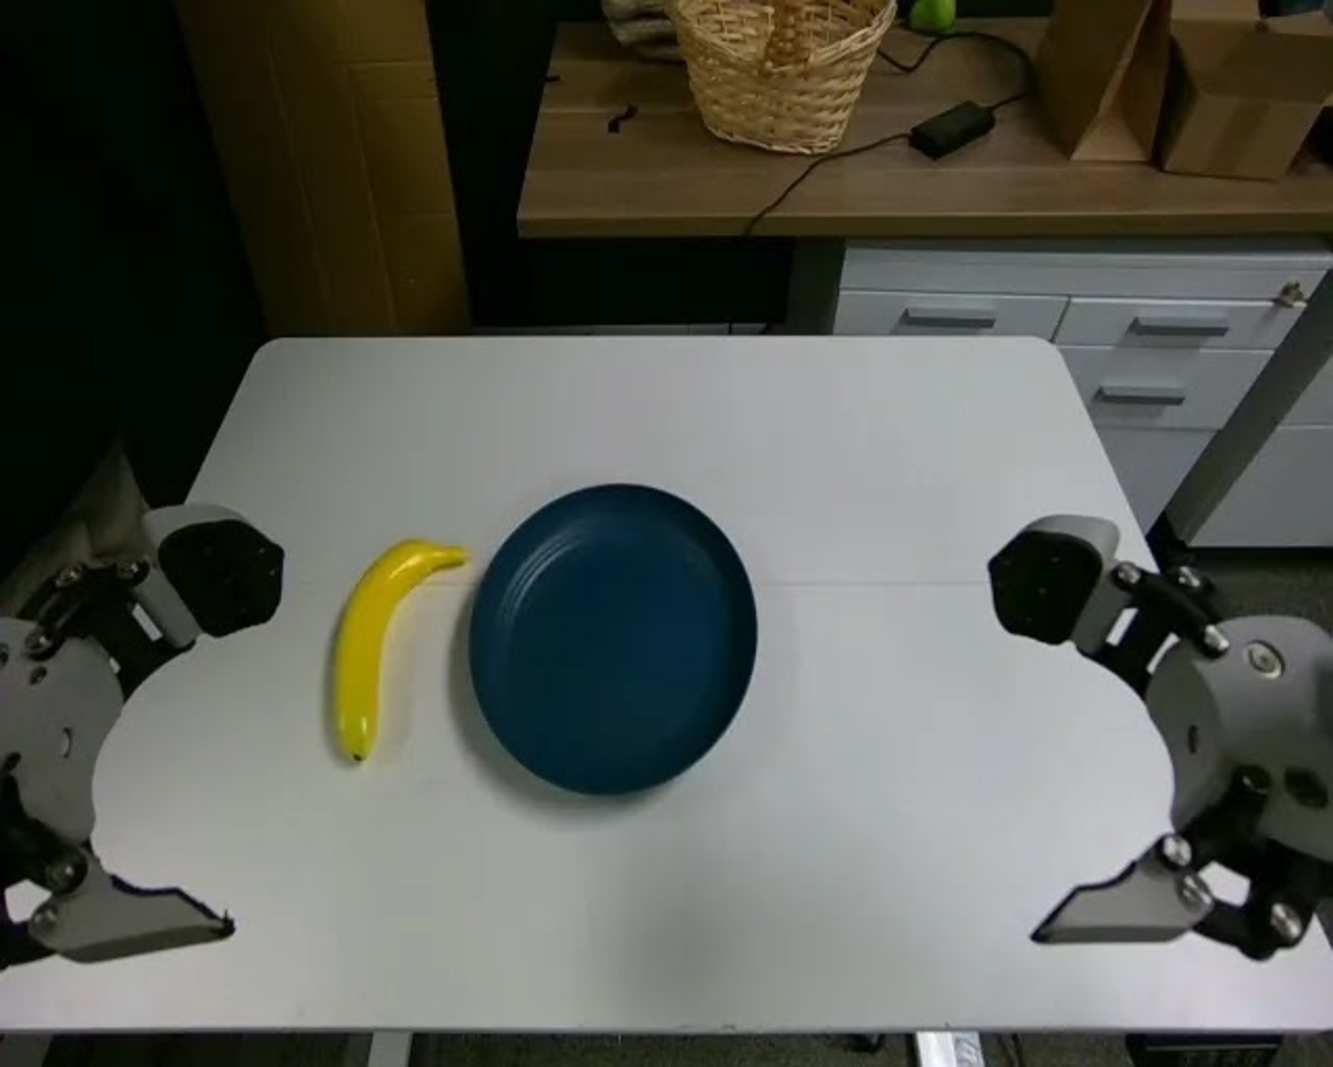
\includegraphics[width=3.2cm]{figures/agibot_seen/task1_r26_v1.pdf} & \centering\scriptsize{The left arm picks up the Banana on the table and places it in the Blue Plate.} & 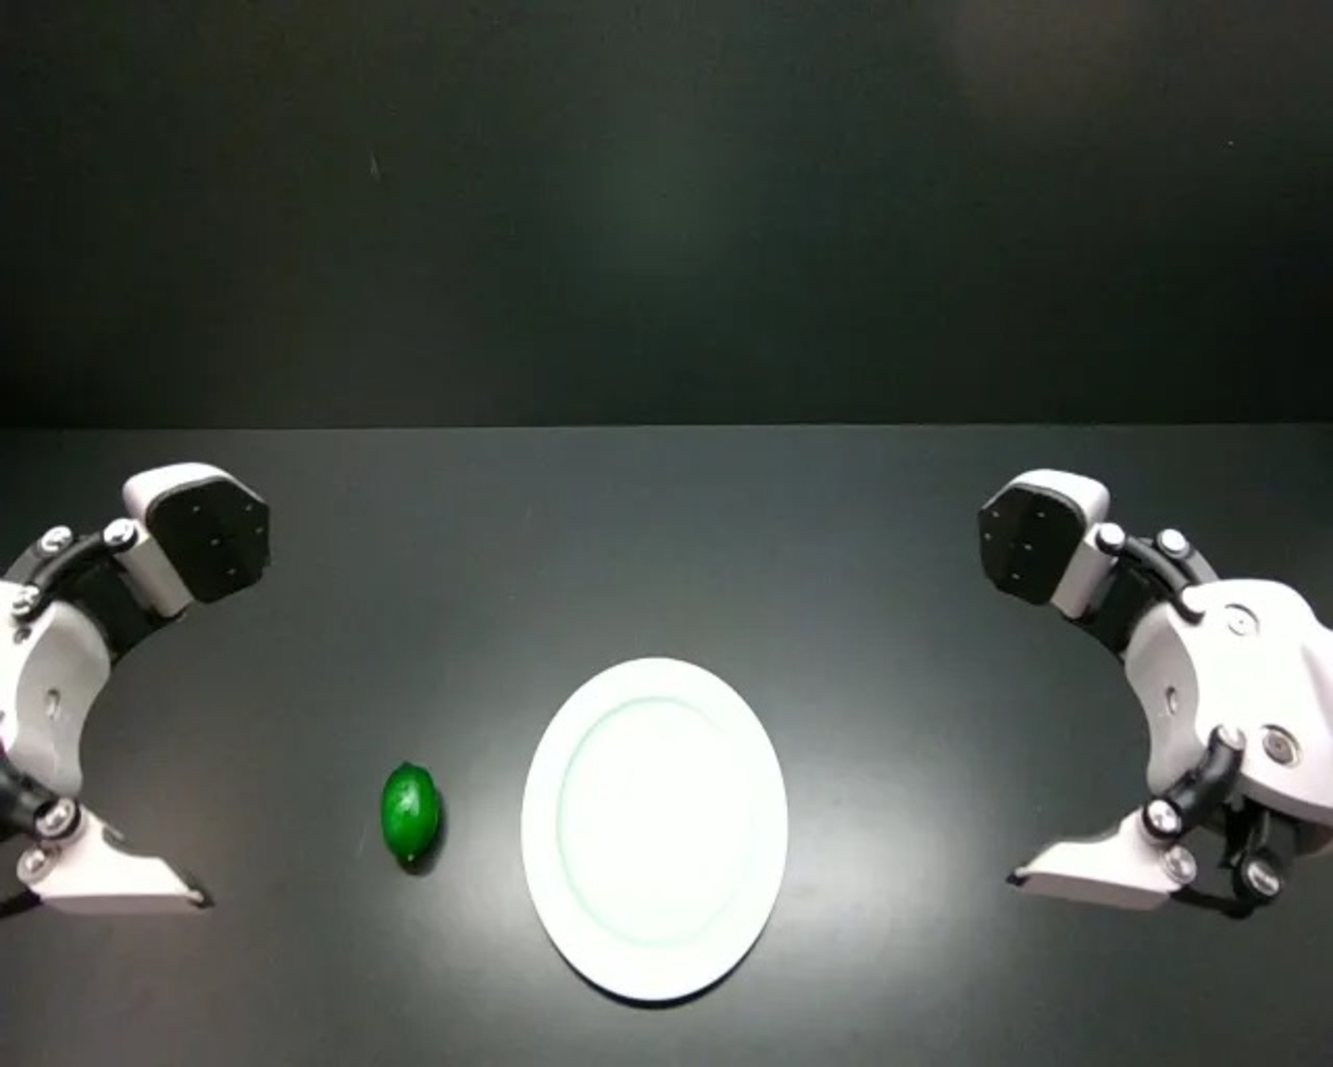
\includegraphics[width=3.2cm]{figures/agibot_seen/task1_r27_v1.pdf} & \centering\scriptsize{The left arm picks up the lime on the table and places it on the light green plate.} & 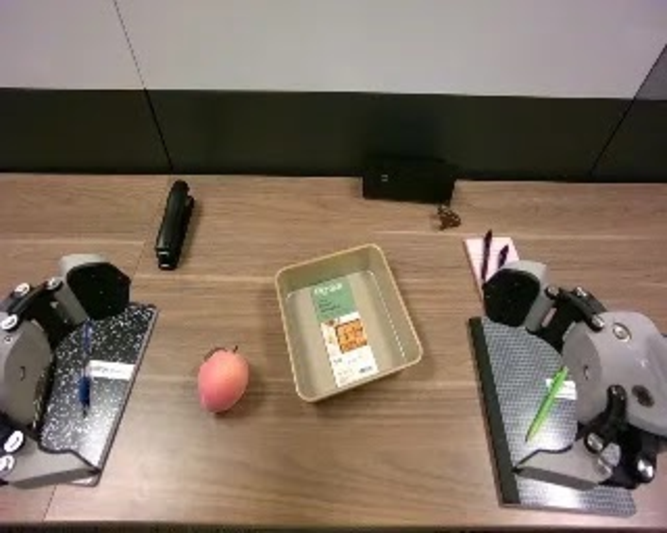
\includegraphics[width=3.2cm]{figures/agibot_seen/task1_r28_v1.pdf} & \centering\scriptsize{The left arm picks up the peach on the table and places it on the baking pan.} & 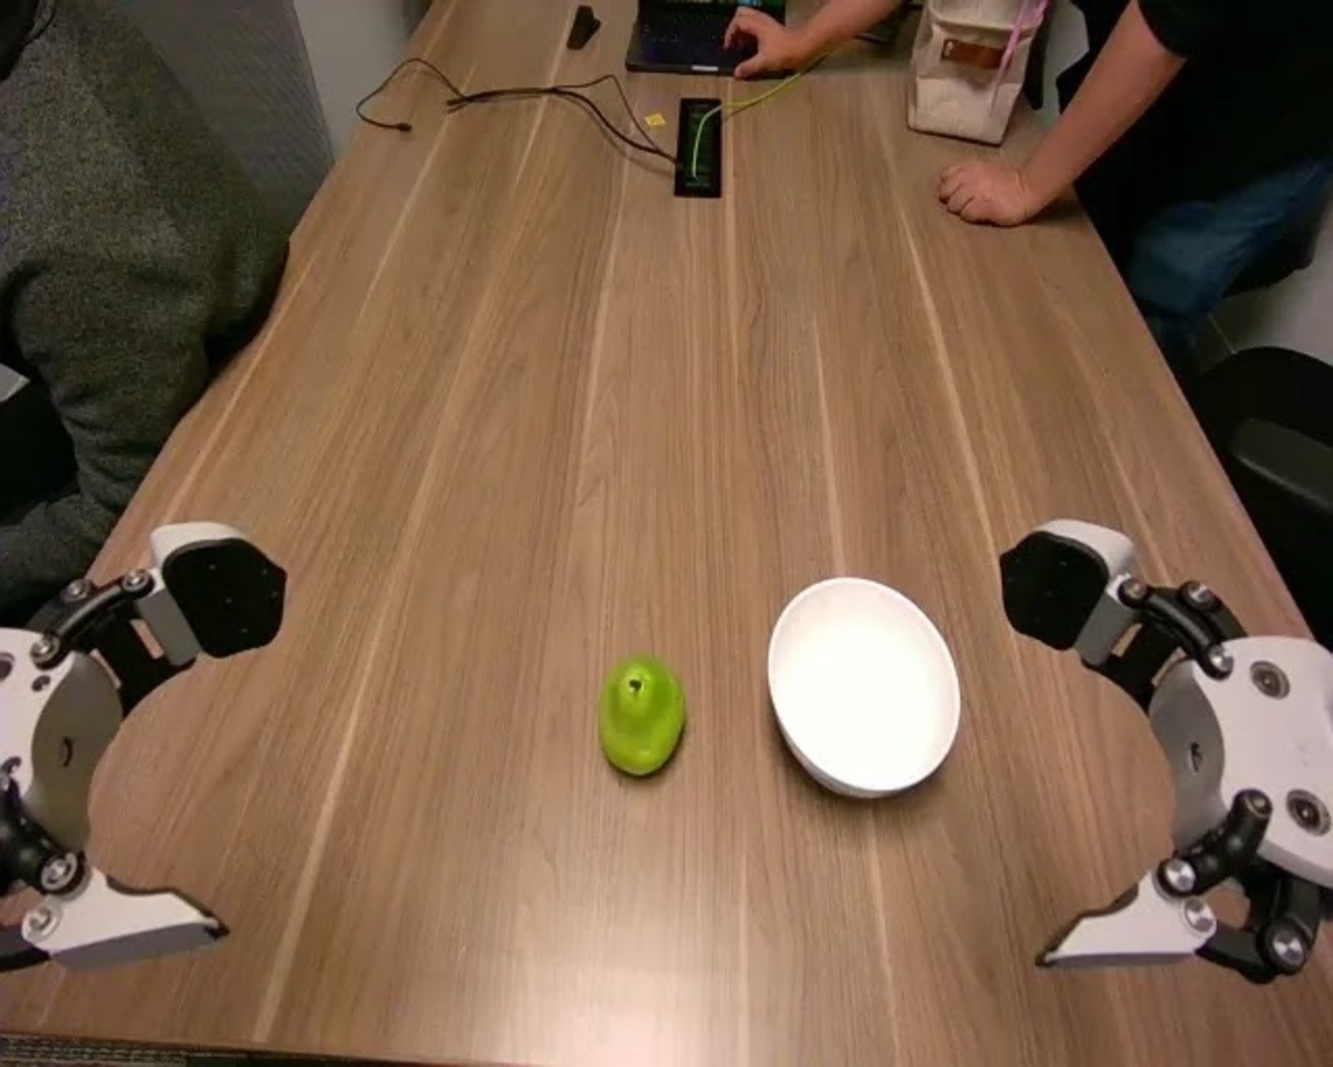
\includegraphics[width=3.2cm]{figures/agibot_seen/task1_r29_v1.pdf} & \centering\arraybackslash\scriptsize{The left arm picks up the green pear on the table and places it on the blue checkered bowl.} \\
\cmidrule(lr){2-11}
\centering\textbf{\shortstack{PnP \\ Easy}} & 2 & \centering\textbf{Taking out Fruit} & 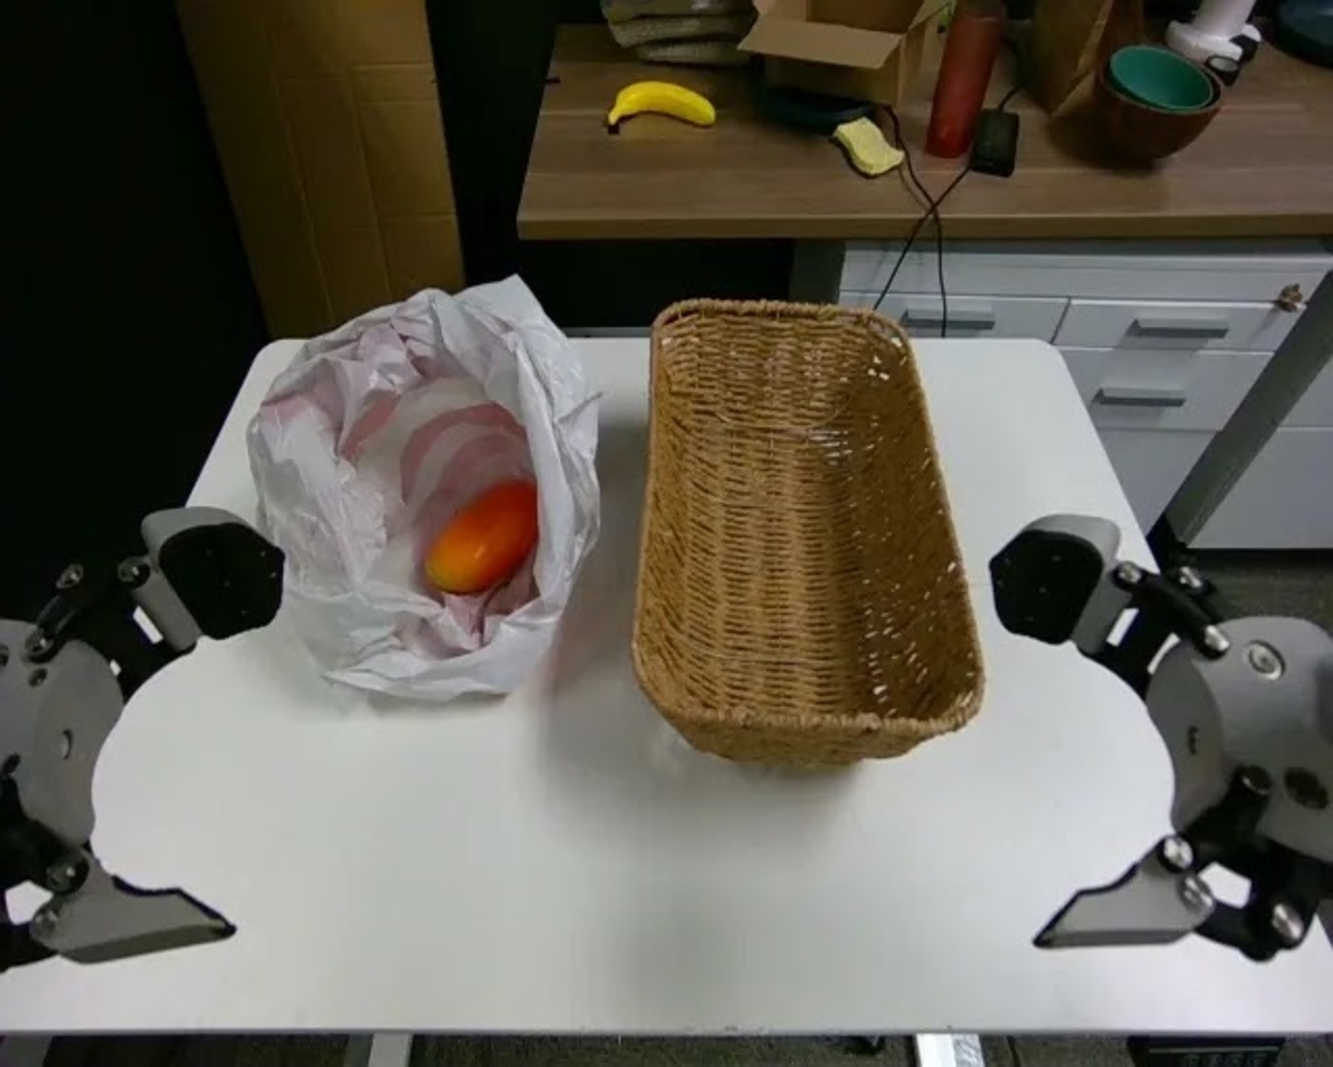
\includegraphics[width=3.2cm]{figures/agibot_seen/task6_r26_v1.pdf} & \centering\scriptsize{The left arm picks up the Mango from the plastic bag and places it into the Wooden Basket} & 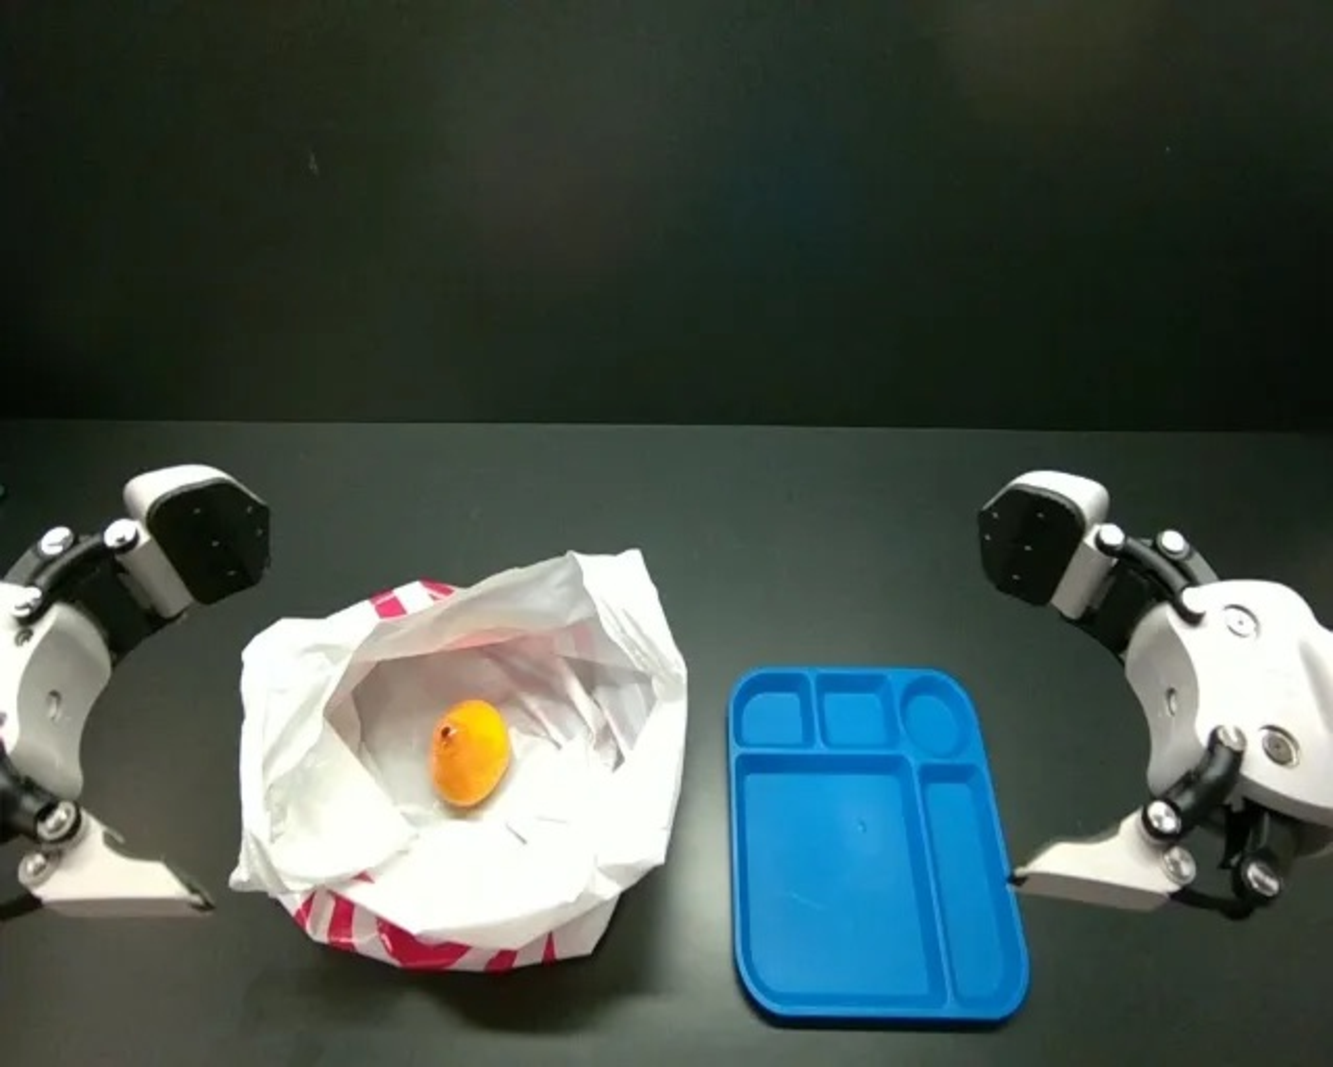
\includegraphics[width=3.2cm]{figures/agibot_seen/task6_r27_v1.pdf} & \centering\scriptsize{The left arm picks up the yellow pear from the plastic bag and places it onto the blue tray.} & 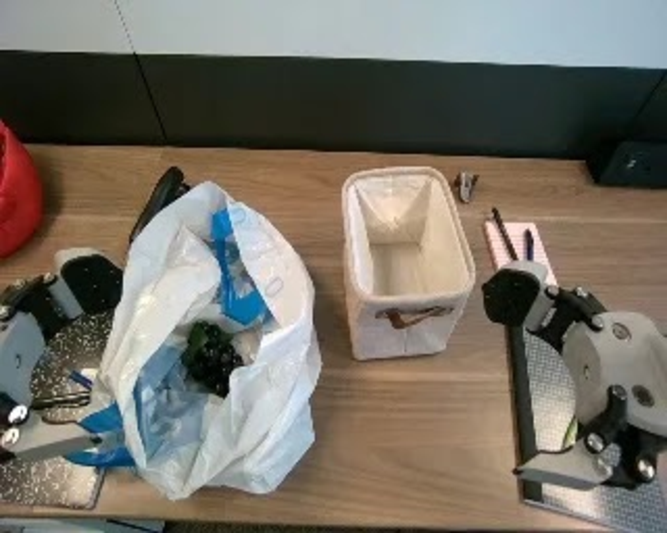
\includegraphics[width=3.2cm]{figures/agibot_seen/task6_r28_v1.pdf} & \centering\scriptsize{The left arm picks up the purple grapes from the plastic bag and places it into the brown basket.} & 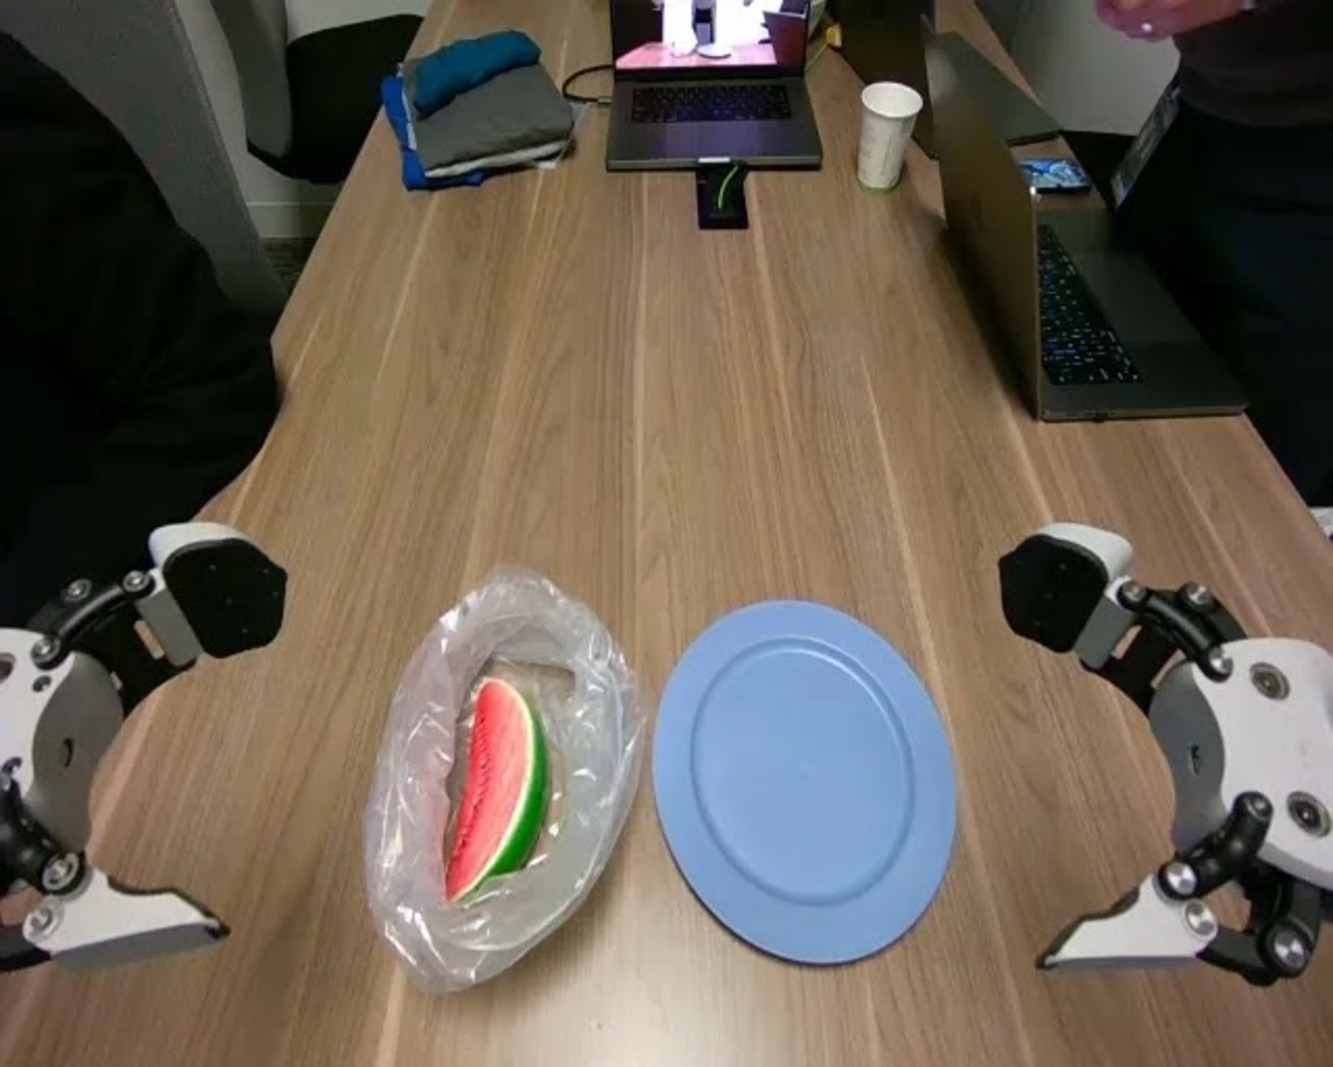
\includegraphics[width=3.2cm]{figures/agibot_seen/task6_r29_v1.pdf} & \centering\arraybackslash\scriptsize{The left arm picks up the watermelon from the plastic bag and places it onto the Blue Plate.} \\
\cmidrule(lr){2-11}
 & 3 & \centering\textbf{Wipe the Mess} & 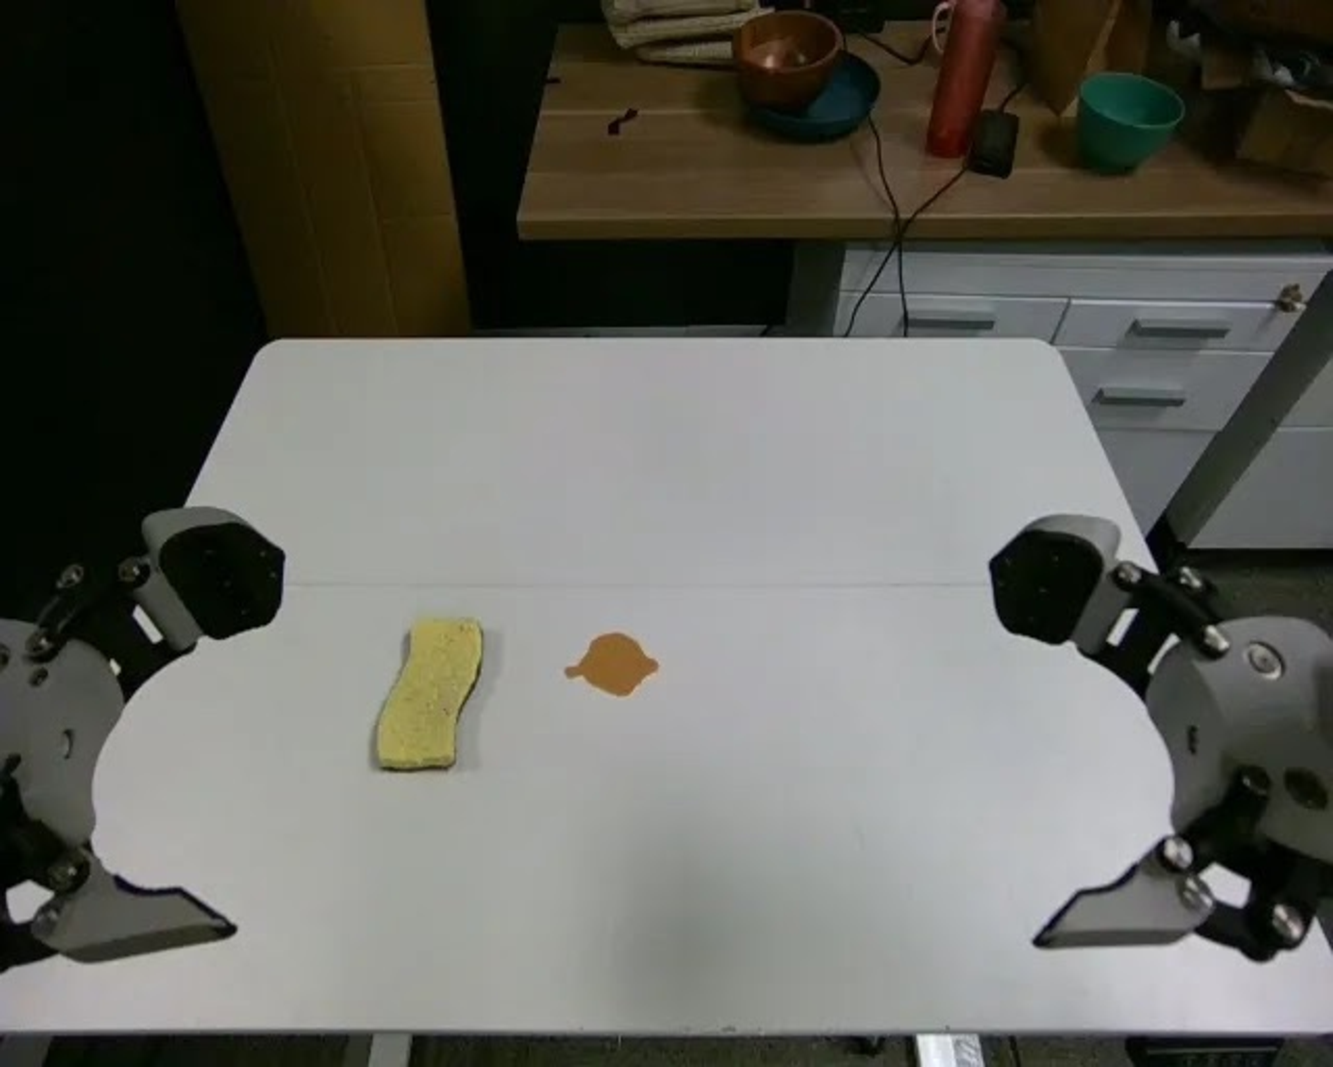
\includegraphics[width=3.2cm]{figures/agibot_seen/task9_r26_v1.pdf} & \centering\scriptsize{The left arm uses a sponge to wipe the coffee spill off the table.} & 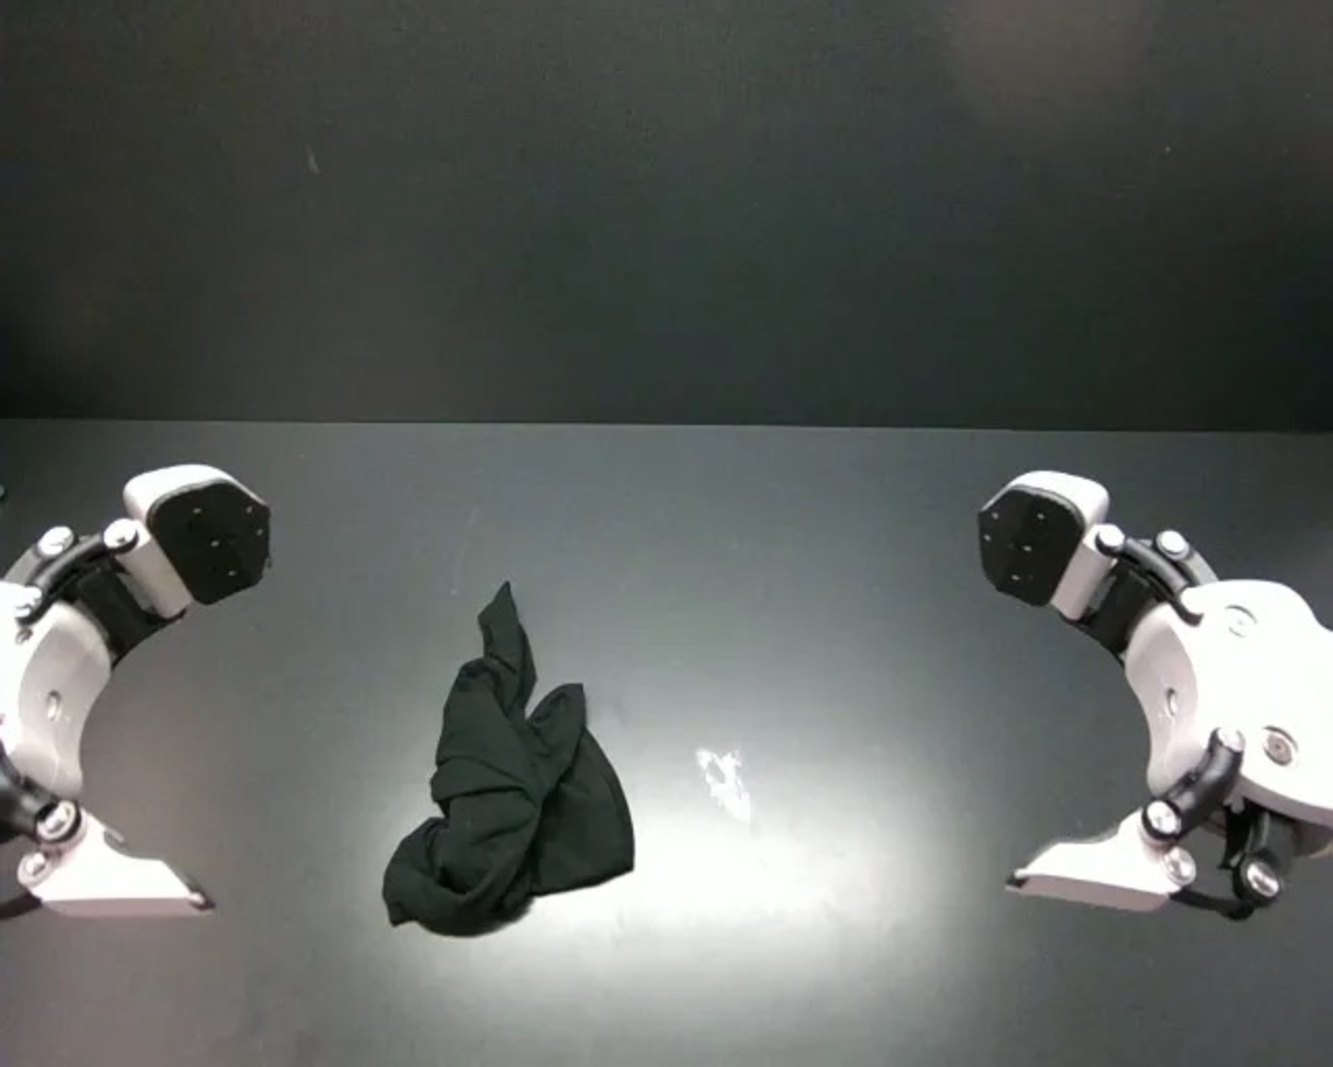
\includegraphics[width=3.2cm]{figures/agibot_seen/task9_r27_v1.pdf} & \centering\scriptsize{The left arm used a black cloth to wipe the white powder off the table.} & 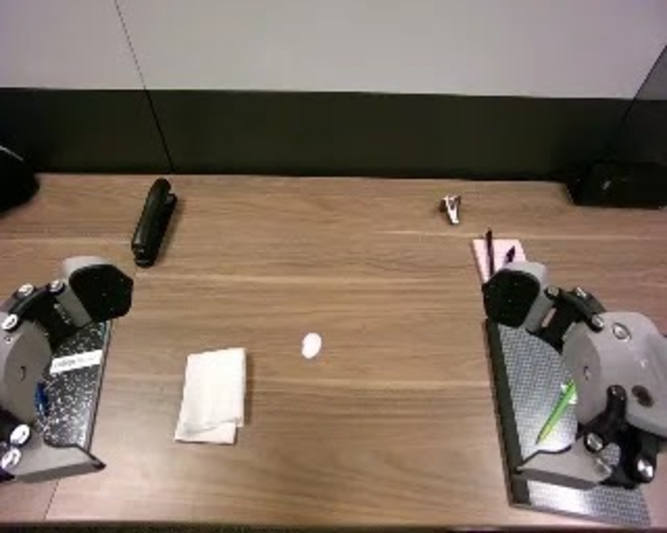
\includegraphics[width=3.2cm]{figures/agibot_seen/task9_r28_v1.pdf} & \centering\scriptsize{The left arm uses a napkin to wipe the creamer spill off the table.} & 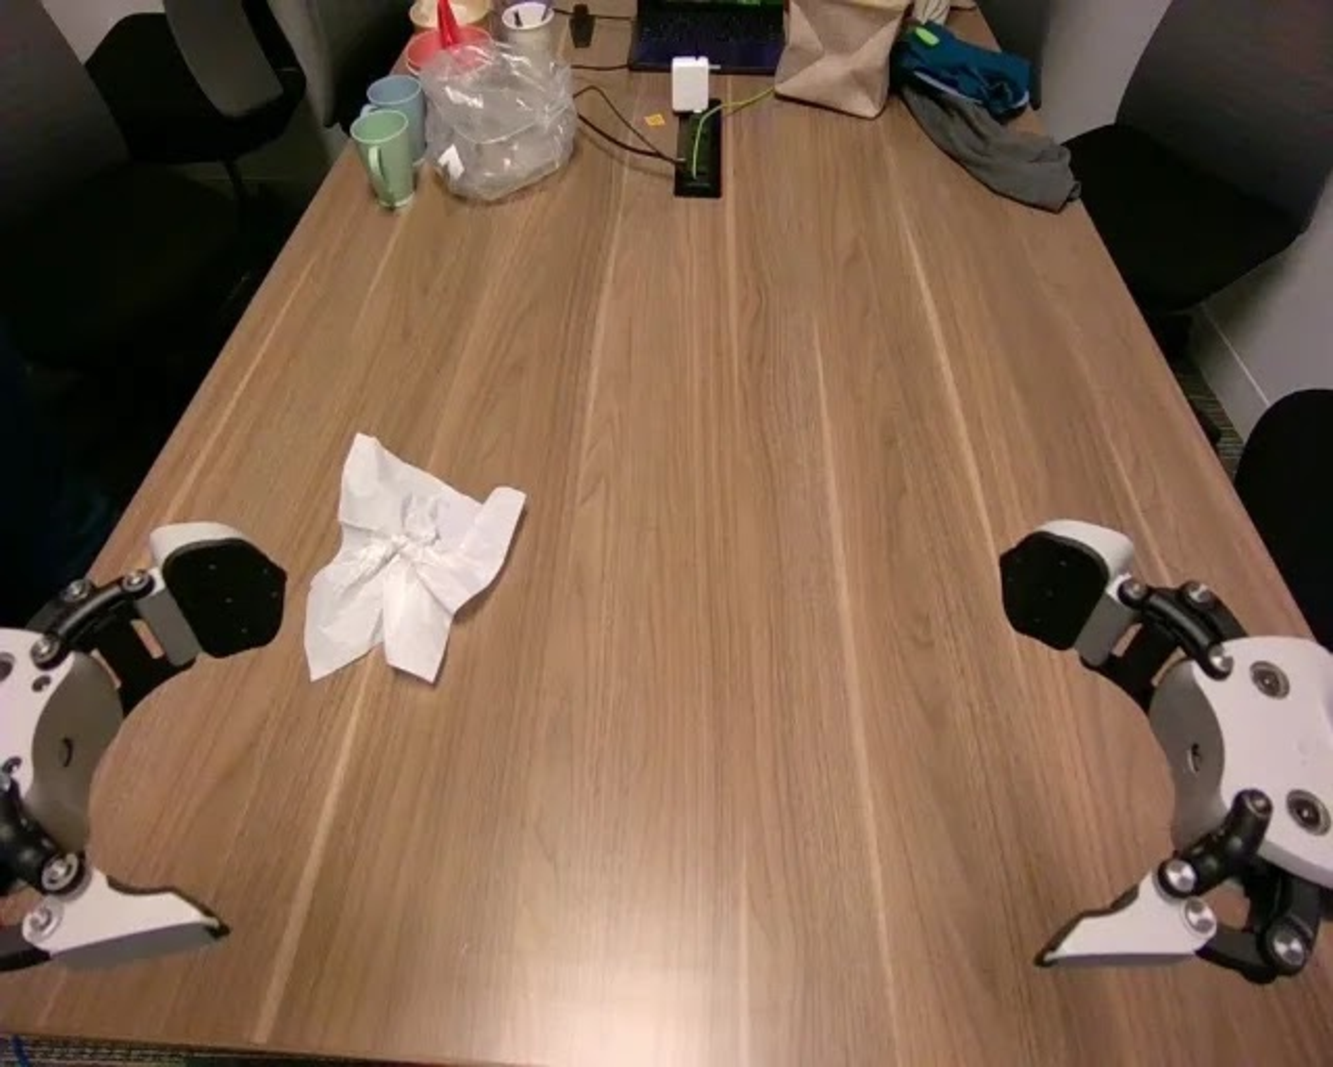
\includegraphics[width=3.2cm]{figures/agibot_seen/task9_r29_v1.pdf} & \centering\arraybackslash\scriptsize{The left arm used a paper towel to wipe the water off the table.} \\
\midrule
 & 4 & \centering\textbf{PnP Fork/Spoon} & 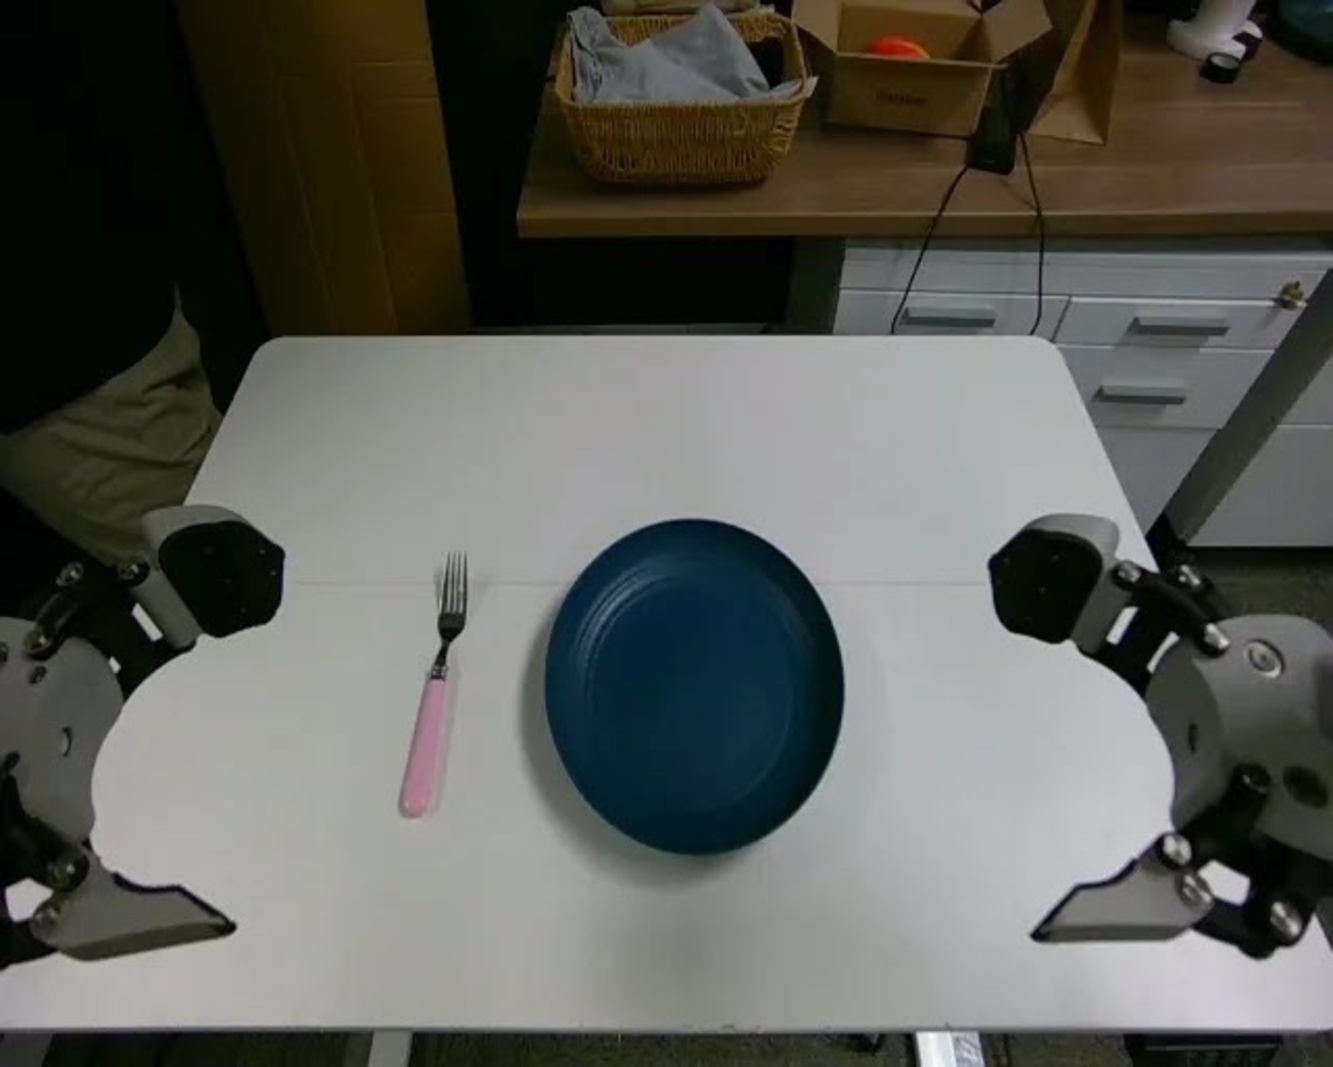
\includegraphics[width=3.2cm]{figures/agibot_seen/task5_r26_v1.pdf} & \centering\scriptsize{The left arm picks up the Pink Fork from the table and places it onto the blue plate.} & 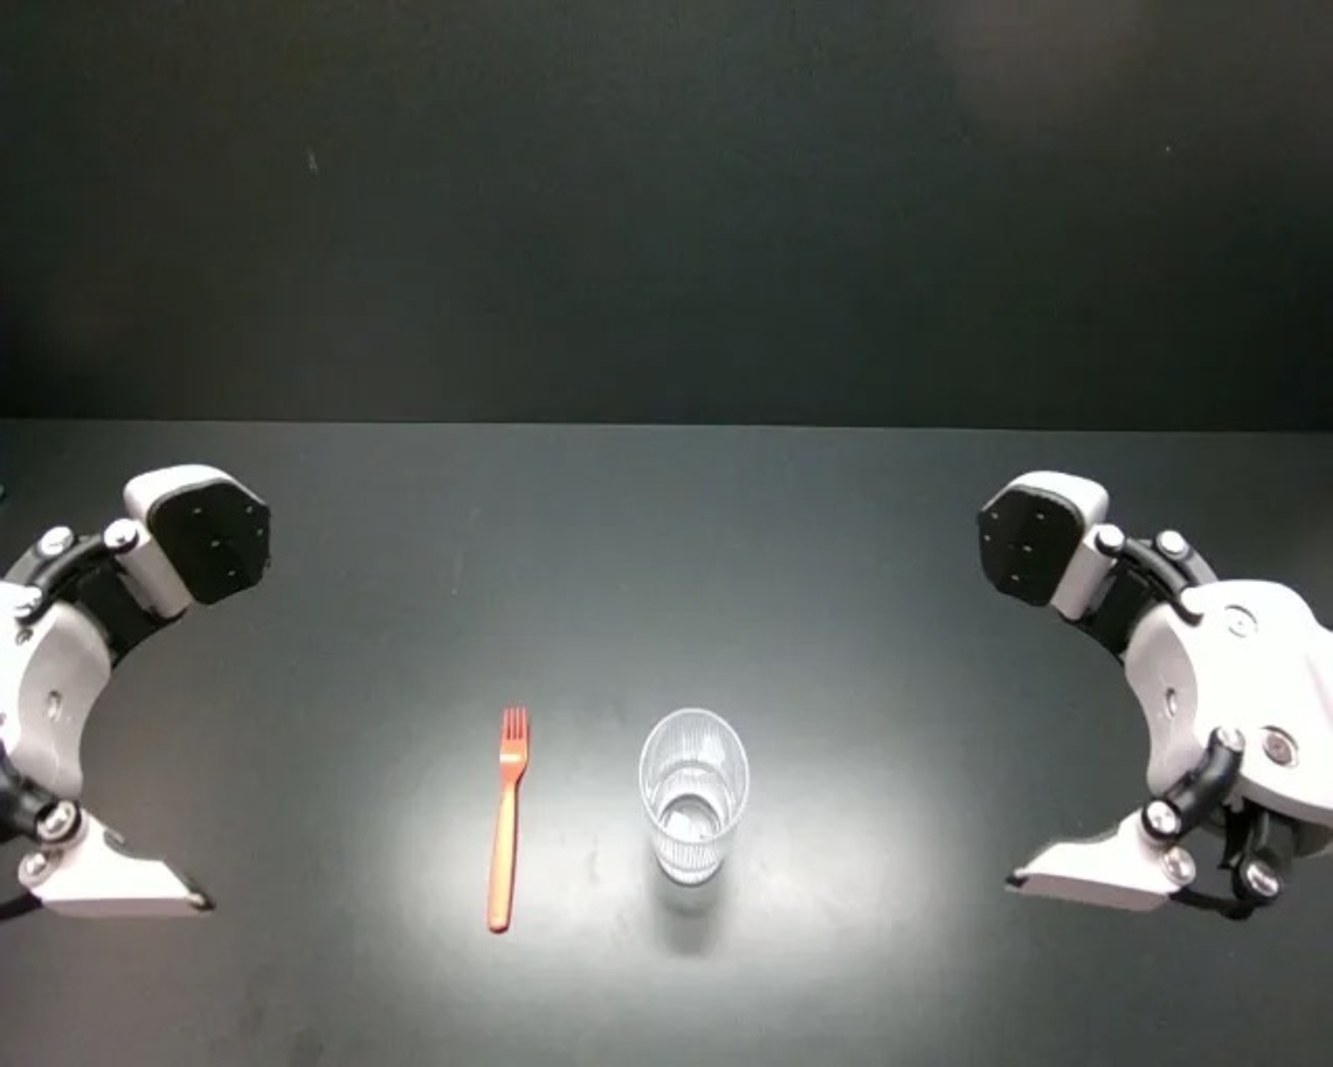
\includegraphics[width=3.2cm]{figures/agibot_seen/task5_r27_v1.pdf} & \centering\scriptsize{The left arm picks up the orange fork from the table and places it into the glass cup} & 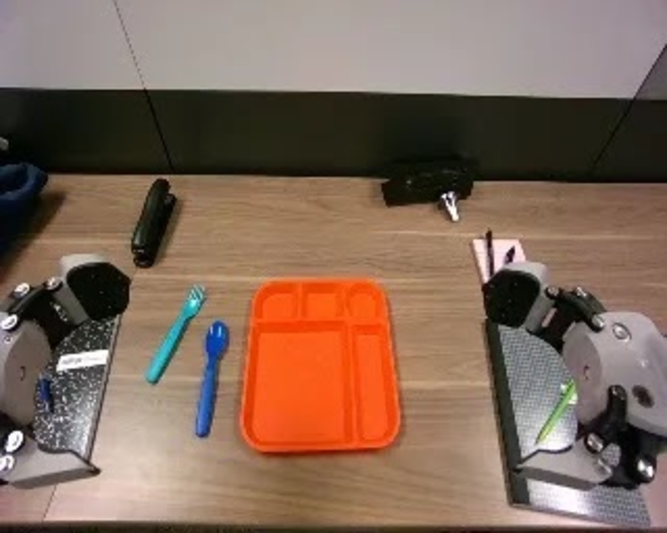
\includegraphics[width=3.2cm]{figures/agibot_seen/task5_r28_v1.pdf} & \centering\scriptsize{The left arm picks up the light blue fork from the table and places it onto the orange plate} & 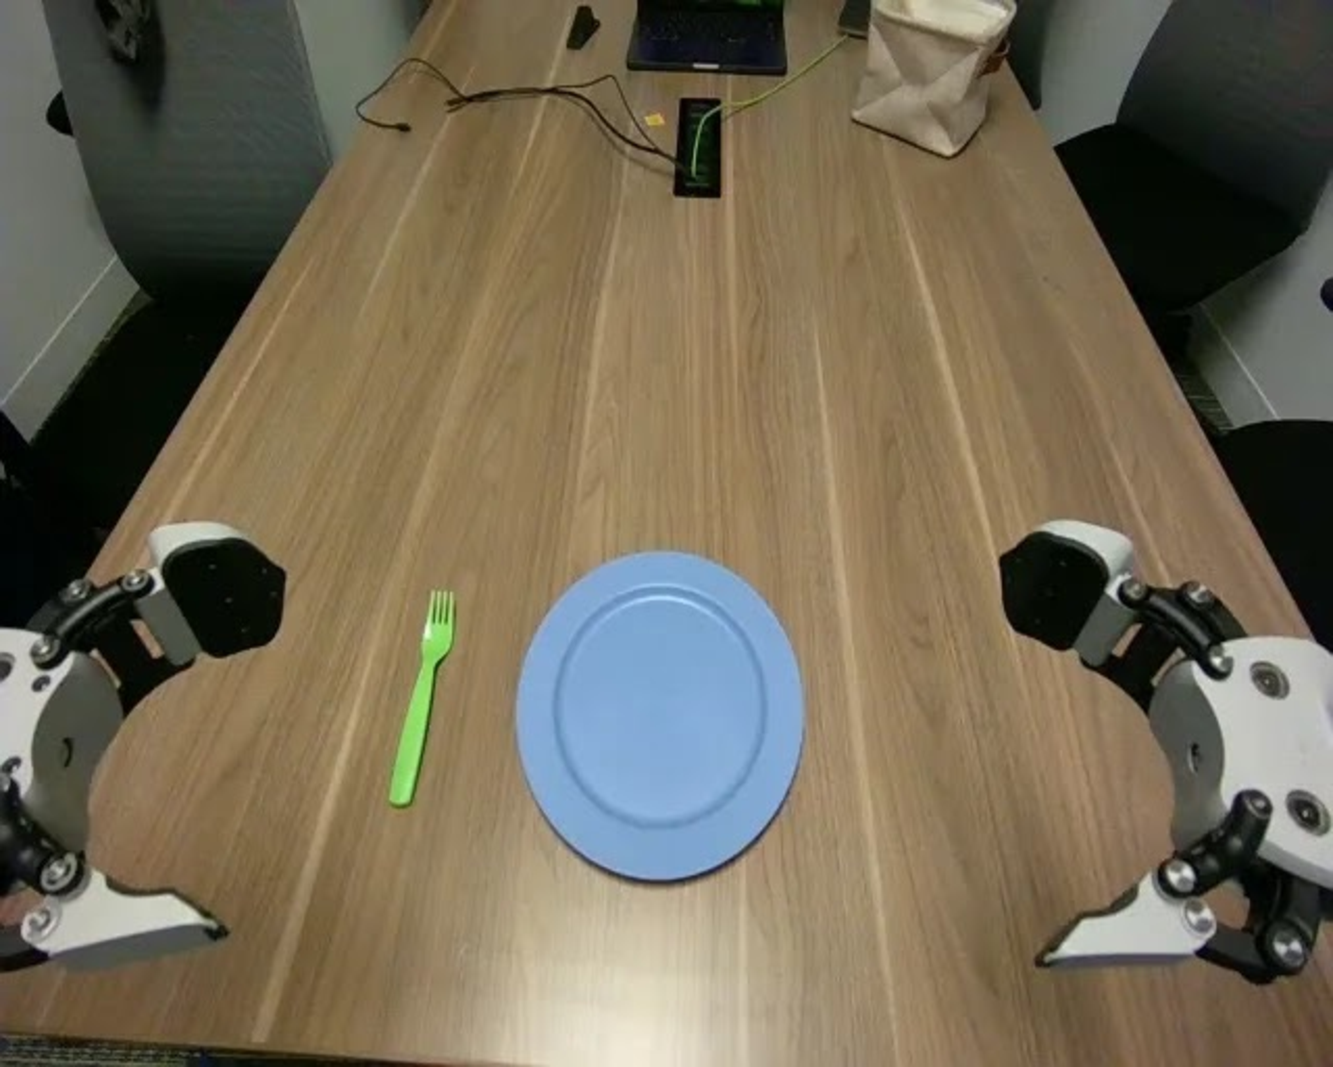
\includegraphics[width=3.2cm]{figures/agibot_seen/task5_r29_v1.pdf} & \centering\arraybackslash\scriptsize{The left arm picks up the green fork from the table and places it into the blue plate.} \\
\cmidrule(lr){2-11}
\multirow{2.3}{*}{\centering\textbf{\shortstack{PnP \\ Hard}}} & 5 & \centering\textbf{Put Pen in Holder} & 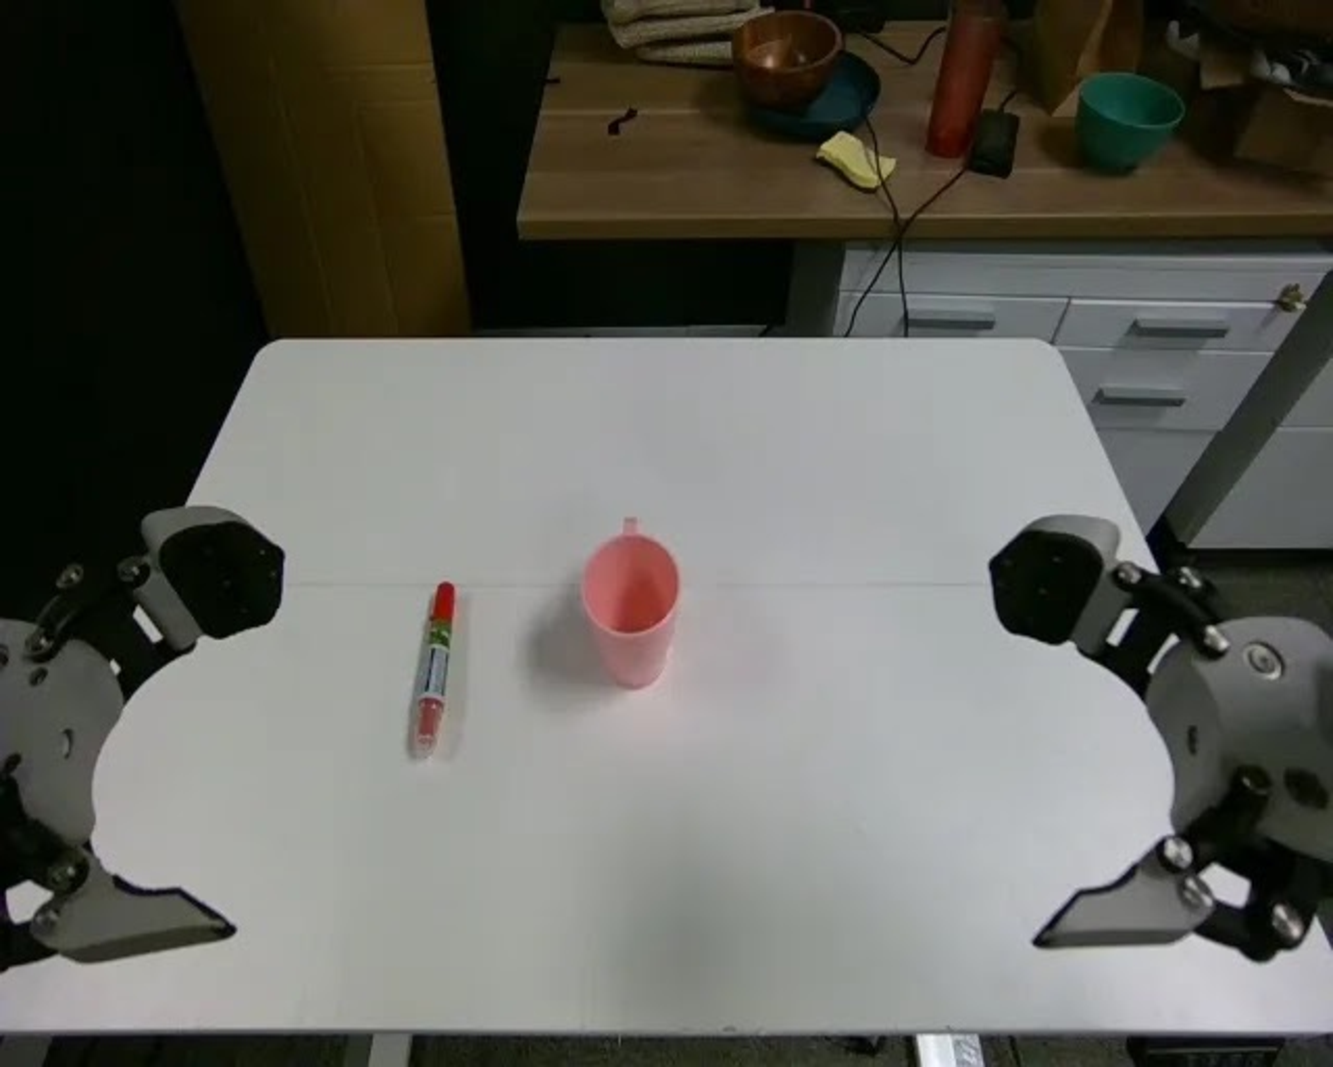
\includegraphics[width=3.2cm]{figures/agibot_seen/task7_r26_v1.pdf} & \centering\scriptsize{The left arm picks up the Red Marker pen from the table and placed it into the pen holder.} & 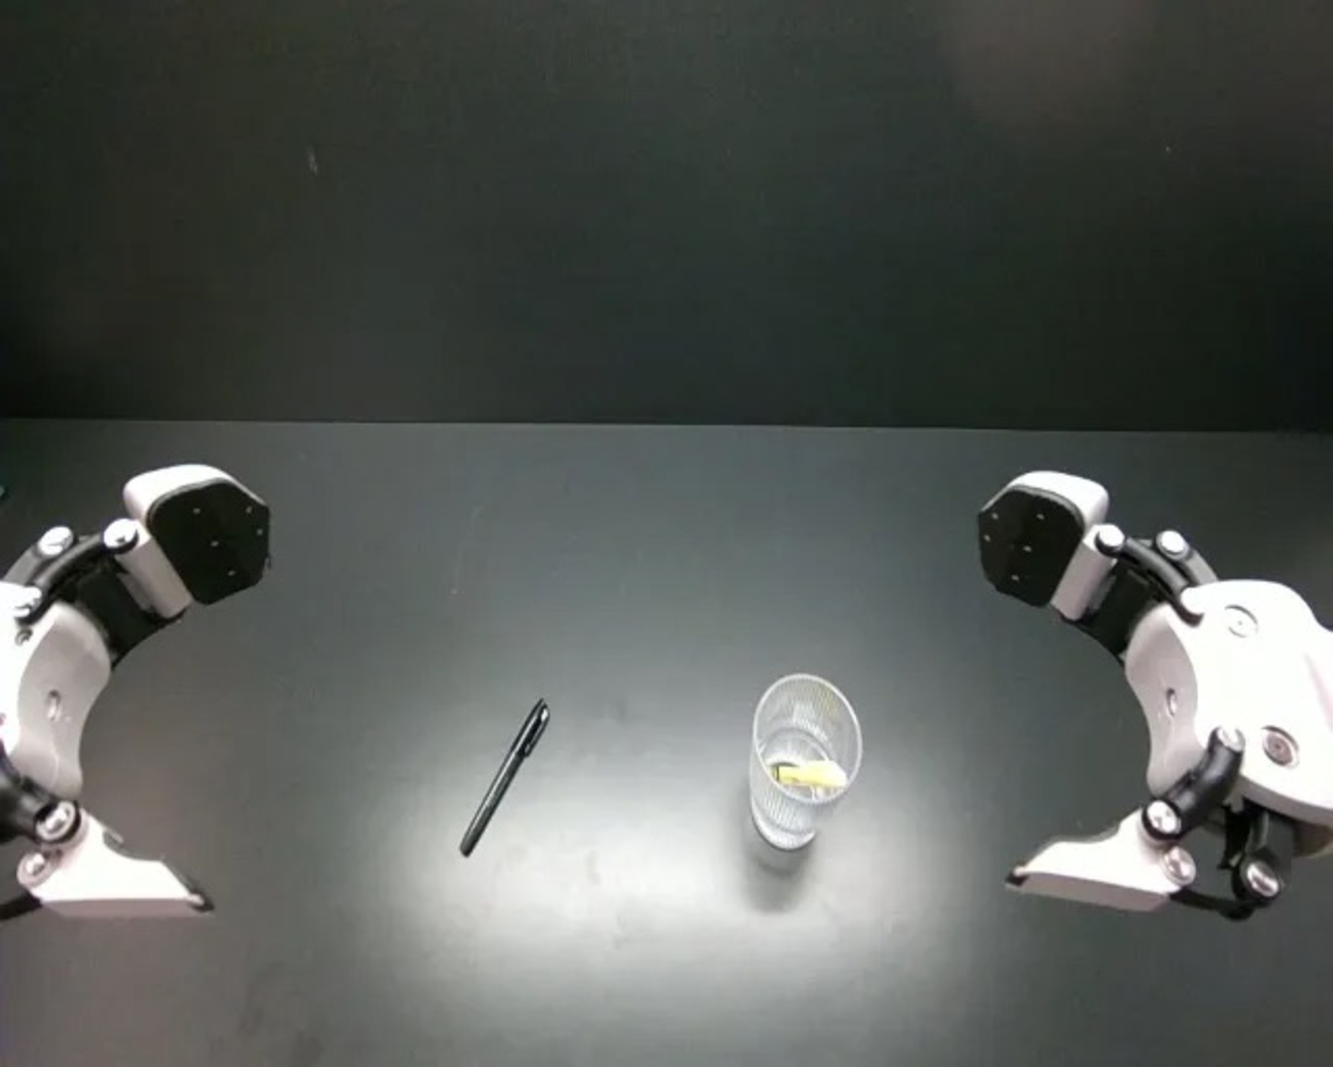
\includegraphics[width=3.2cm]{figures/agibot_seen/task7_r27_v1.pdf} & \centering\scriptsize{The left arm picked up the black marker from the table and placed it into the pen holder.} & 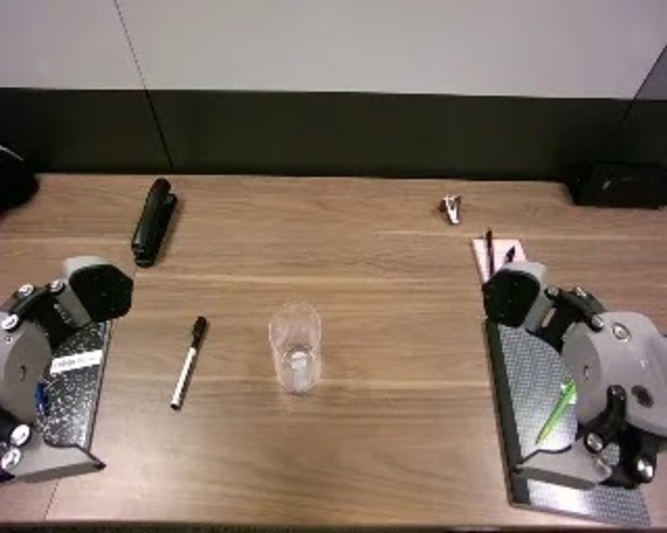
\includegraphics[width=3.2cm]{figures/agibot_seen/task7_r28_v1.pdf} & \centering\scriptsize{The left arm picked up the white marker pen from the table and placed it into the pen holder.} & 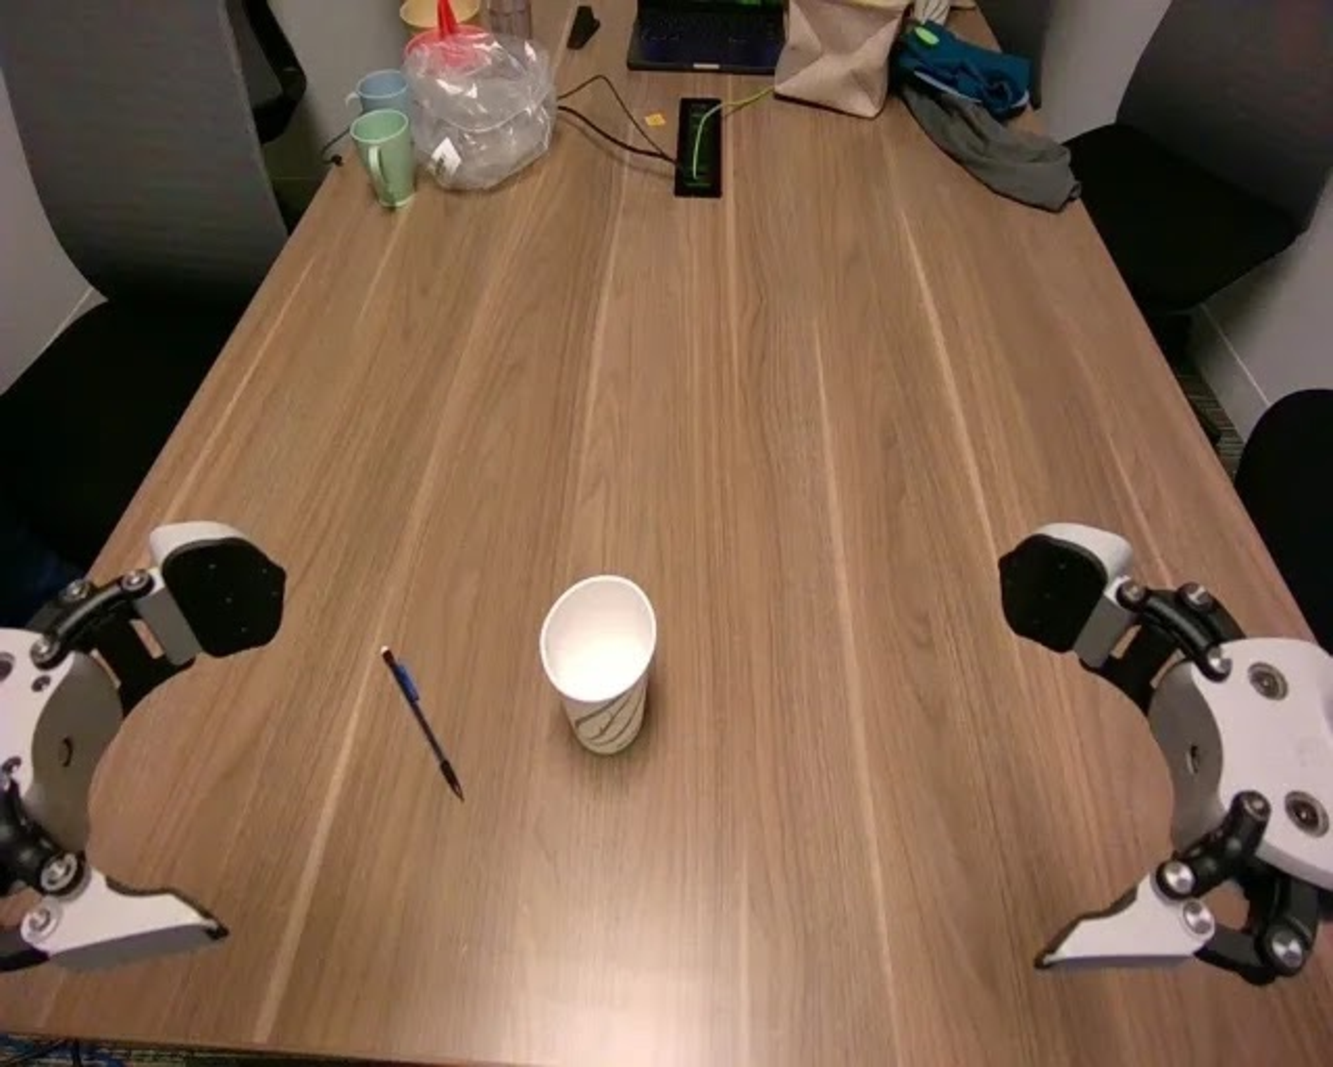
\includegraphics[width=3.2cm]{figures/agibot_seen/task7_r29_v1.pdf} & \centering\arraybackslash\scriptsize{The left arm picked up the mechanical pencil from the table and placed it into the pen holder.} \\
\cmidrule(lr){2-11}
 & 6 & \centering\textbf{Put Cup on Coaster} & 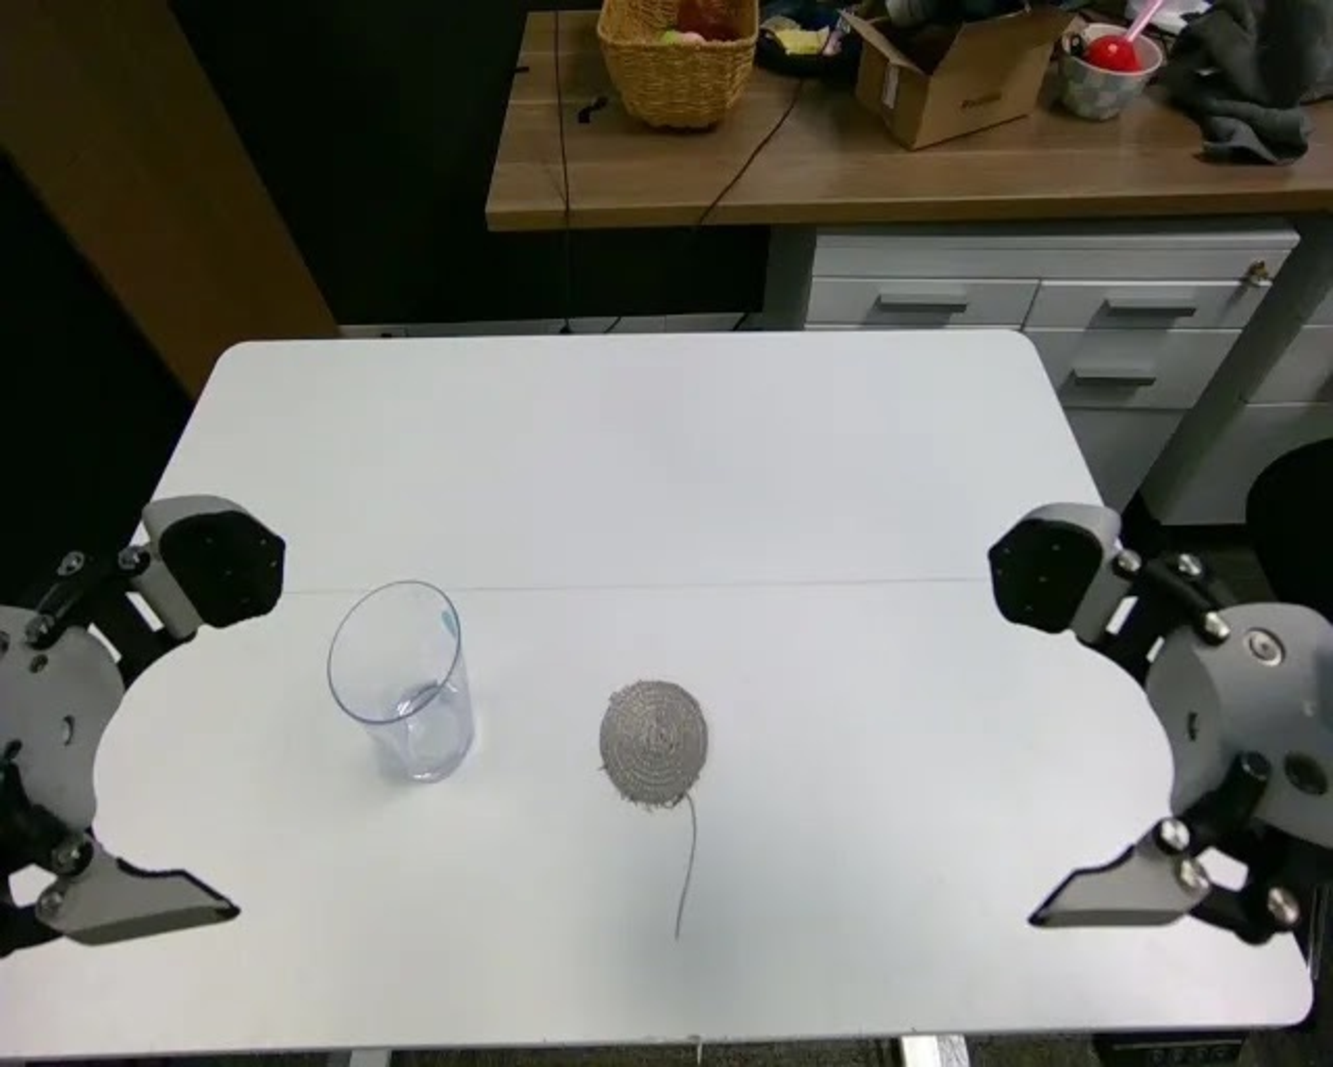
\includegraphics[width=3.2cm]{figures/agibot_seen/task8_r26_v1.pdf} & \centering\scriptsize{The left arm picks up the clear cup from the table and places it on the grey coaster.} & 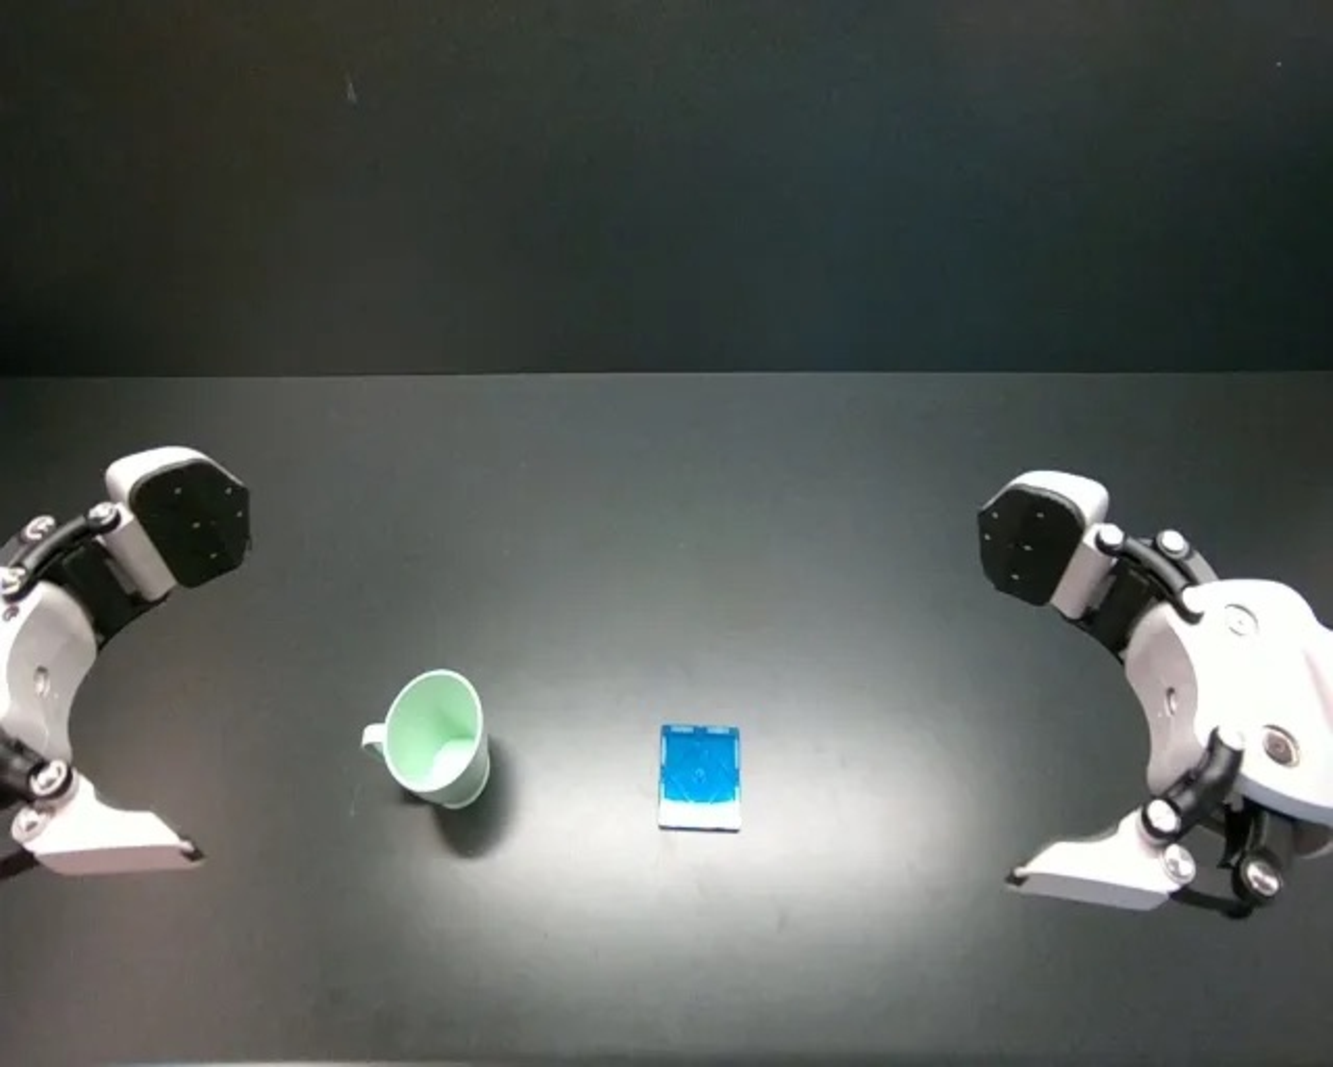
\includegraphics[width=3.2cm]{figures/agibot_seen/task8_r27_v1.pdf} & \centering\scriptsize{The left arm picks up the plastic cup from the table and places it on the blue coaster.} & 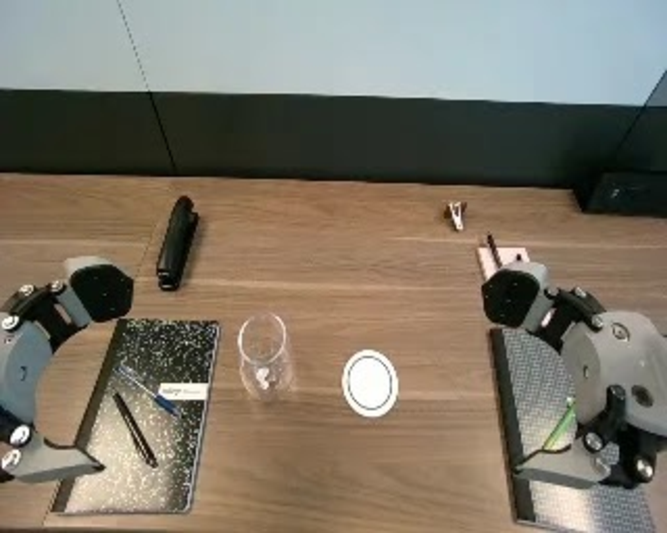
\includegraphics[width=3.2cm]{figures/agibot_seen/task8_r28_v1.pdf} & \centering\scriptsize{The left arm picks up the plastic cup from the table and places it on the white coaster.} & 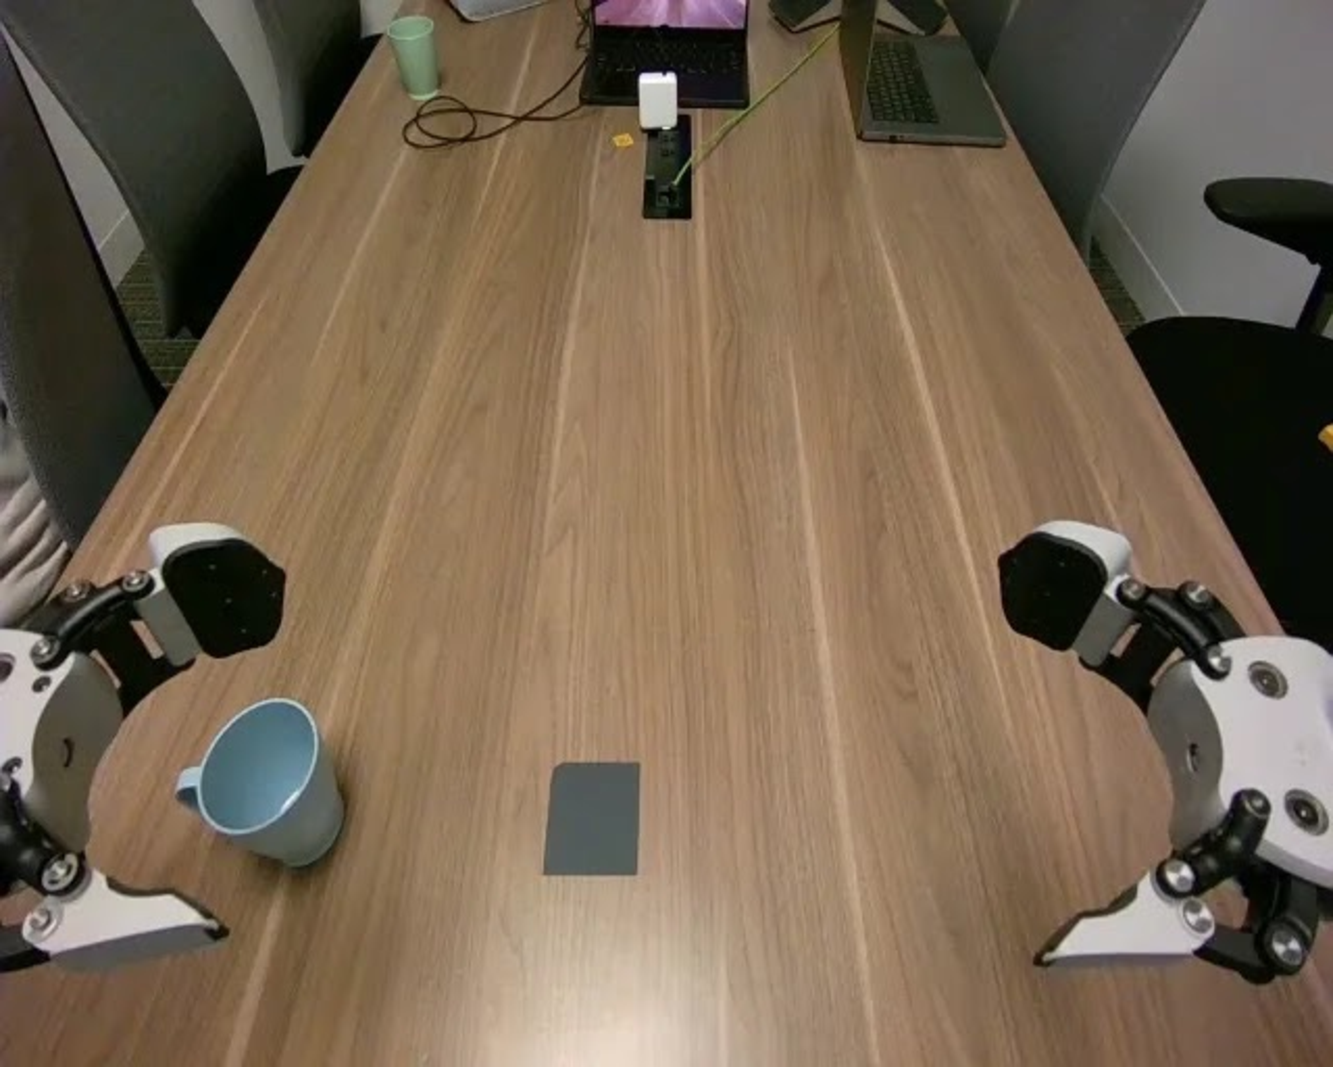
\includegraphics[width=3.2cm]{figures/agibot_seen/task8_r29_v1.pdf} & \centering\arraybackslash\scriptsize{The left arm picks up the pink cup from the table and places it on the gray coaster.} \\
\cmidrule(lr){2-11}
 & 7 & \centering\textbf{Stack Bowls/Cups} & 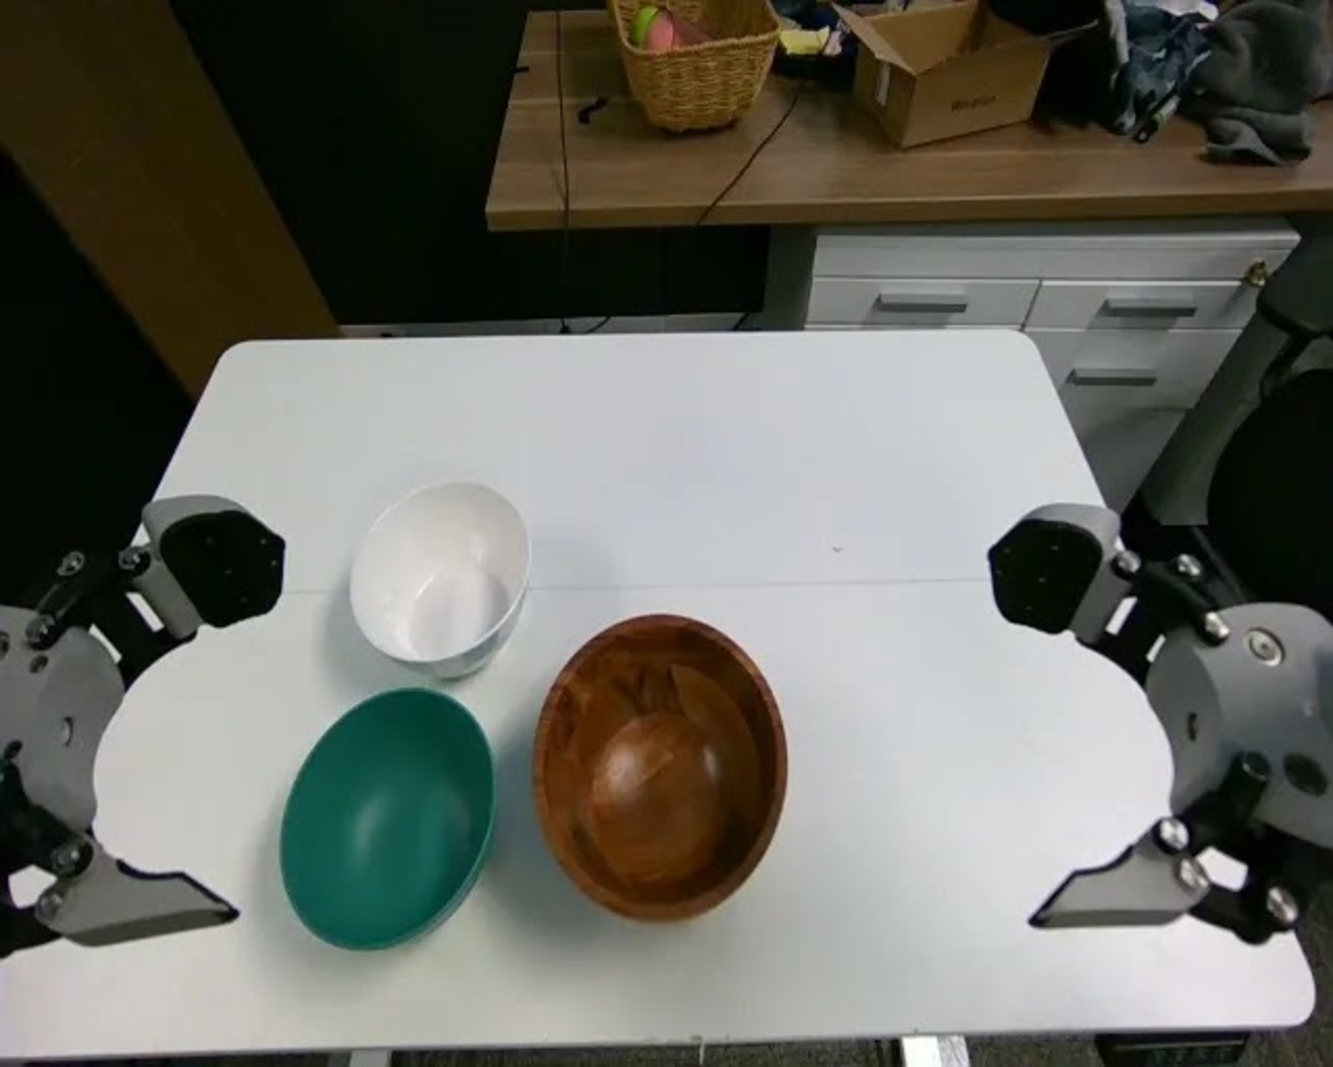
\includegraphics[width=3.2cm]{figures/agibot_seen/task10_r26_v1.pdf} & \centering\scriptsize{The robot reaches to grip the green bowl, moves it to the middle wooden bowl, and releases it to stack. It then reaches to grip the white bowl, moves it to the same location, and releases it onto the stack.} & 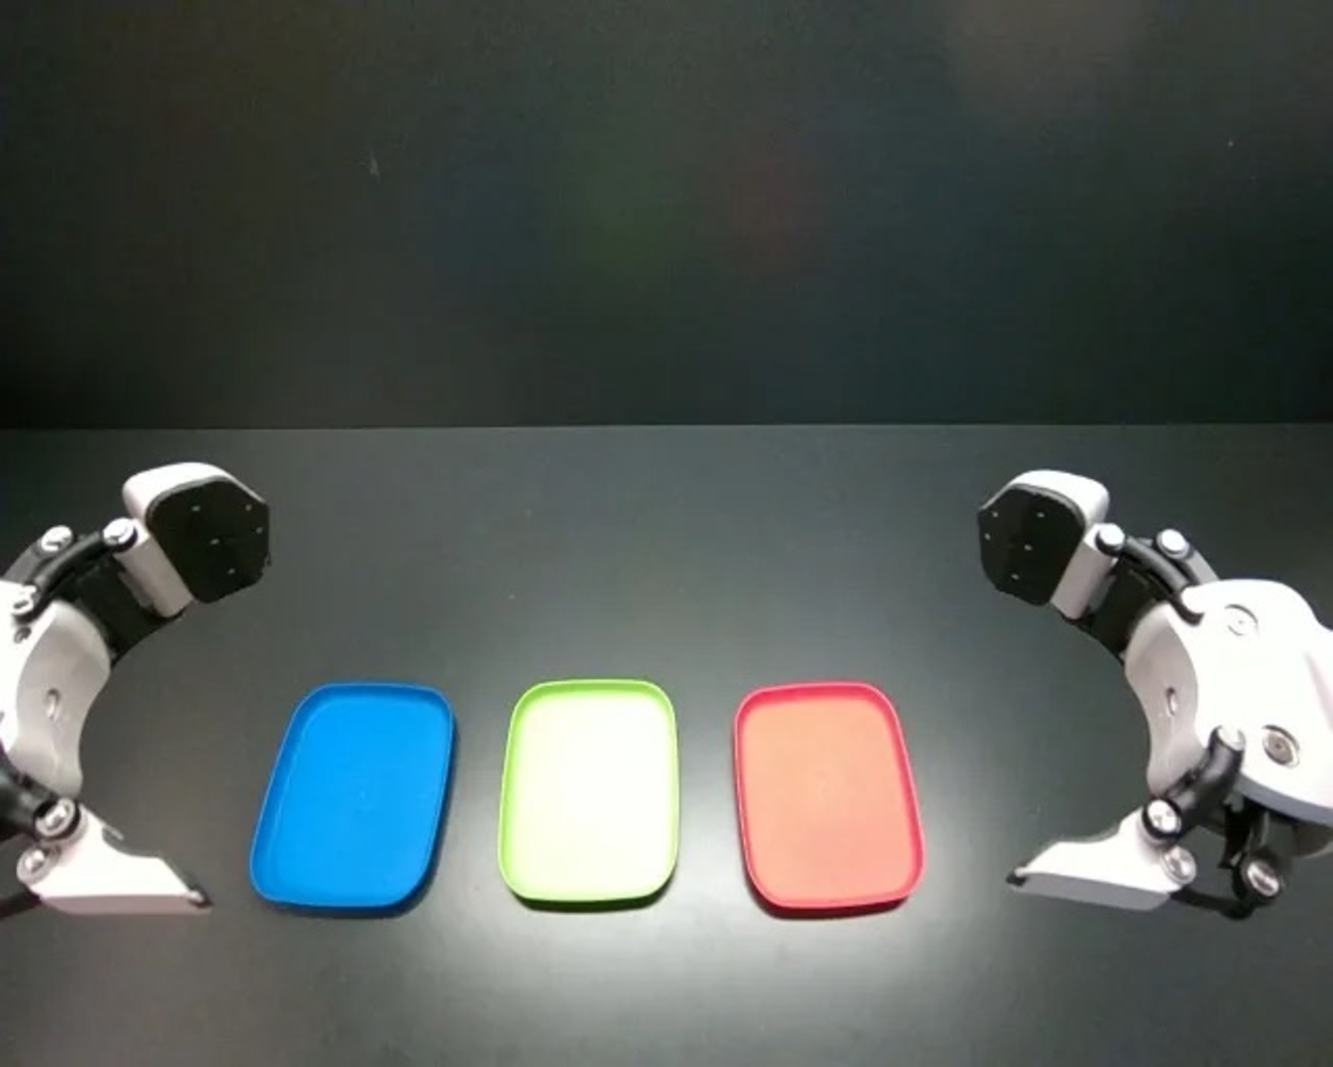
\includegraphics[width=3.2cm]{figures/agibot_seen/task10_r27_v1.pdf} & \centering\scriptsize{The robot reaches its left arm to grip the blue plate, moves it to the middle light green plate, and releases it to stack. It then reaches its right arm to grip the red plate, moves it over the middle stack of plates, and releases it to finish the task.} & 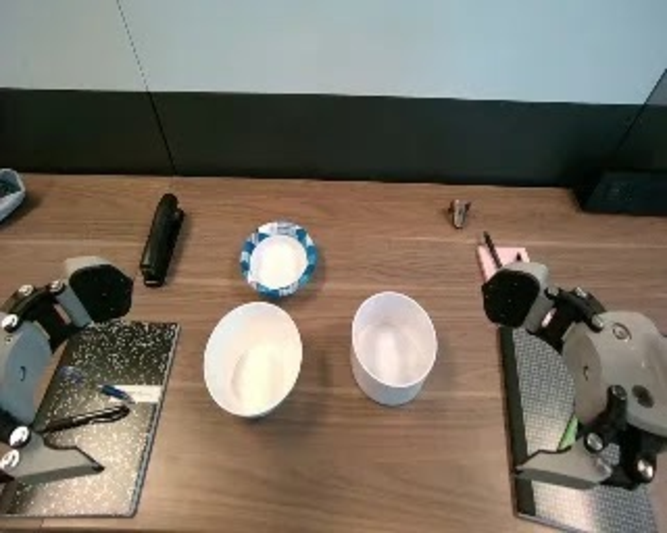
\includegraphics[width=3.2cm]{figures/agibot_seen/task10_r28_v1.pdf} & \centering\scriptsize{The robot reaches its left arm to grip the paper bowl, moves it over the middle white bowl, and releases it to stack. It then reaches its left arm to grip the blue checkered bowl, moves it over the stack, and releases it to finish the task.} & 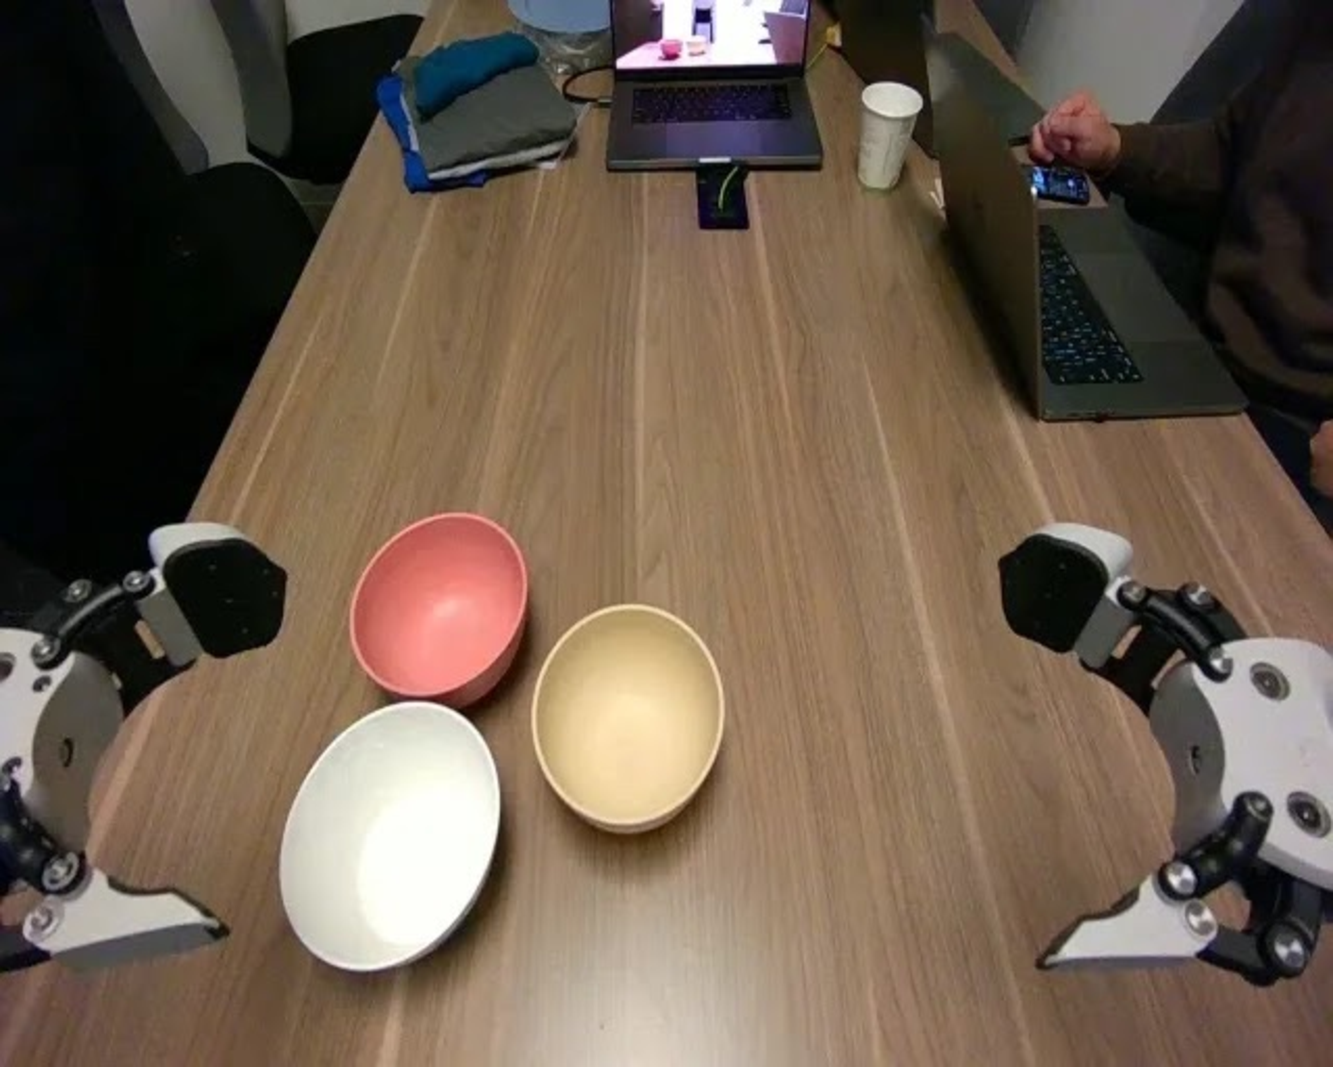
\includegraphics[width=3.2cm]{figures/agibot_seen/task10_r29_v1.pdf} & \centering\arraybackslash\scriptsize{The robot reaches its left arm to grip the pink bowl, moves it over the middle beige bowl, and releases it to stack. It then reaches its left arm to grip the white bowl, moves it over the stack, and releases it onto the stack.} \\
\midrule
 & 8 & \centering\textbf{Folding Shirts} & 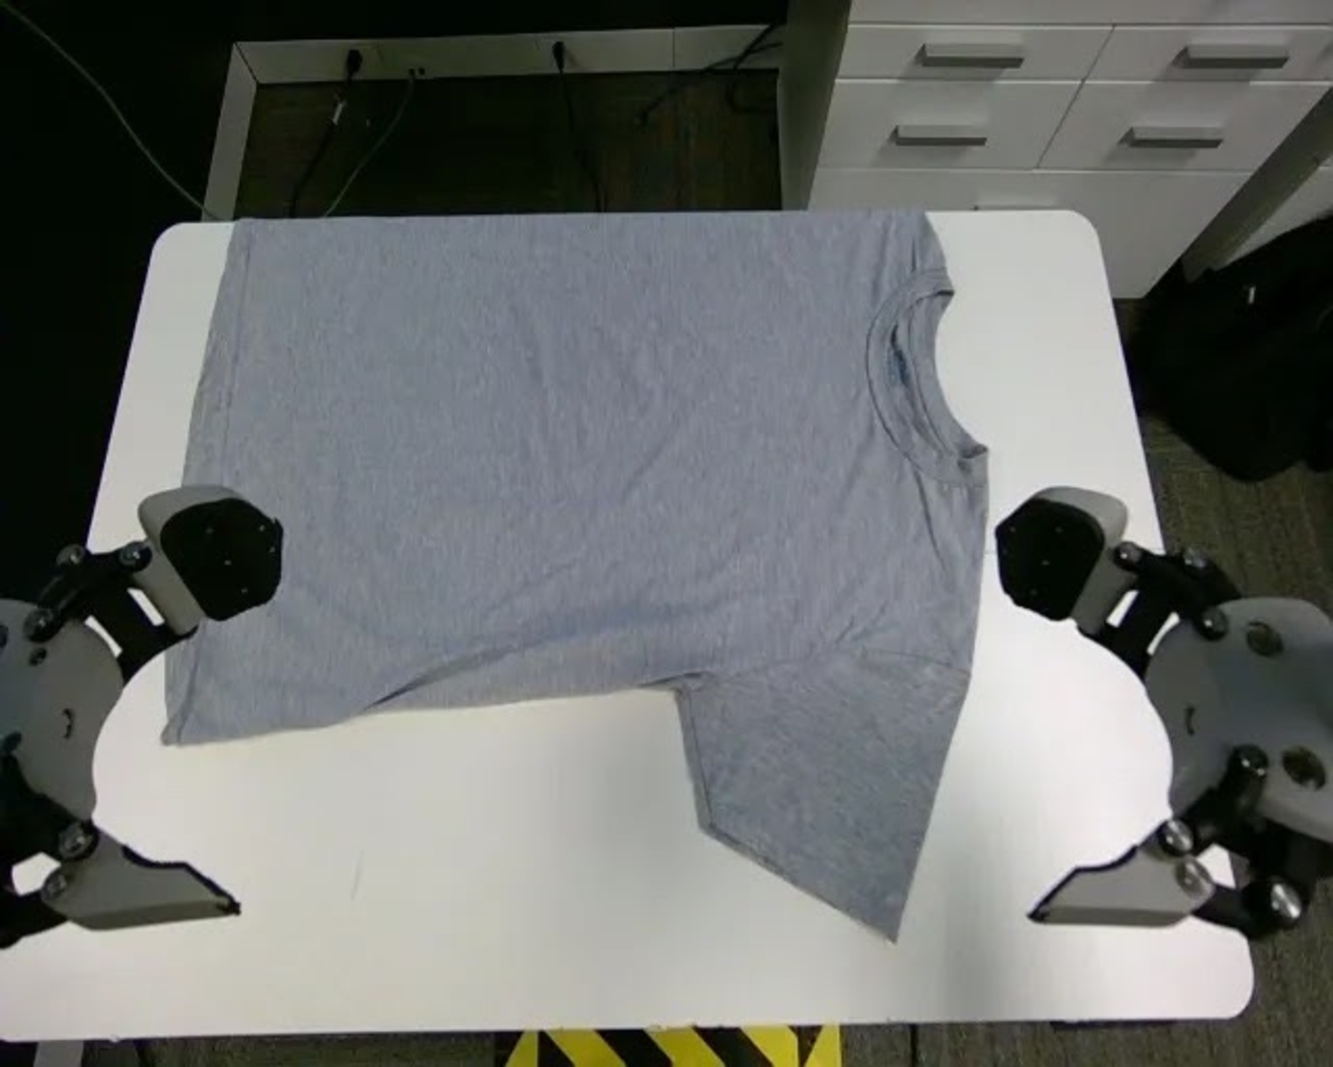
\includegraphics[width=3.2cm]{figures/agibot_seen/task2_r26_v1.pdf} & \centering\scriptsize{Both arms grip the bottom of the light grey short sleeve and fold it toward the middle. They then pull the short sleeve across the table to the edge. Next, both arms grasp the top of the shirt and fold it down to the middle. Finally, the right arm grips the collar and folds it down to complete the task.} & 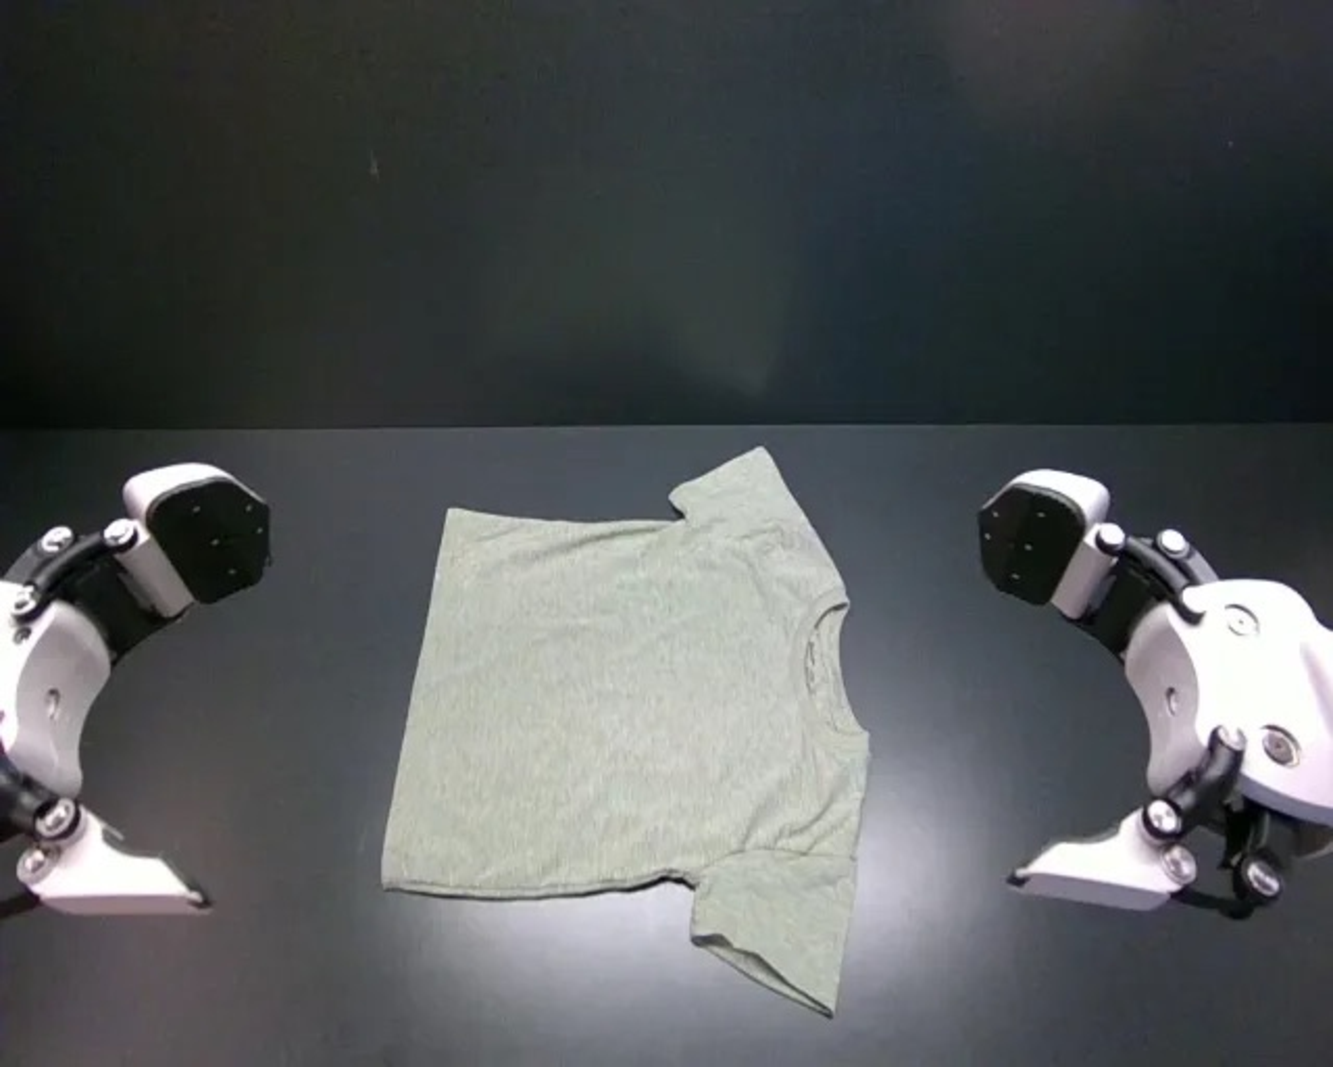
\includegraphics[width=3.2cm]{figures/agibot_seen/task2_r27_v1.pdf} & \centering\scriptsize{Both arms fold the bottom of the green short sleeve to the middle. They then pull the shirt toward the edge of the table. Next, both arms fold the top of the shirt down to the middle. Finally, the right arm grasps the collar and folds it down to complete the task.} & 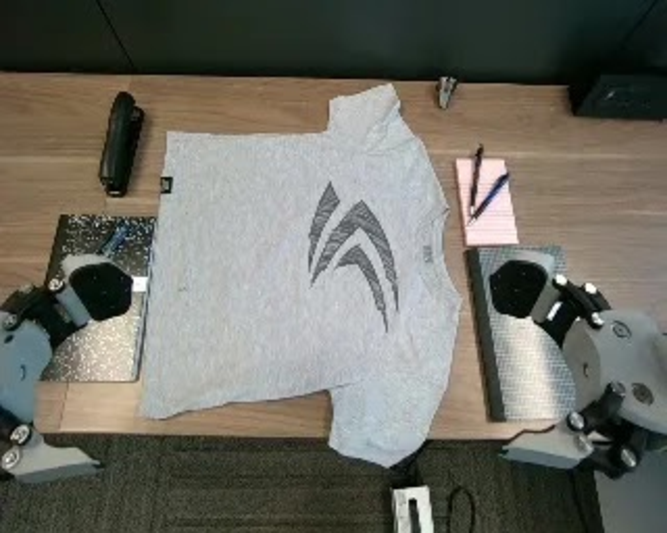
\includegraphics[width=3.2cm]{figures/agibot_seen/task2_r28_v1.pdf} & \centering\scriptsize{Both arms fold the bottom of the logo short sleeve to the middle. They then pull the shirt toward the edge of the table. Next, both arms fold the top of the shirt down to the middle. Finally, the right arm grasps the collar and folds it down to complete the task.} & 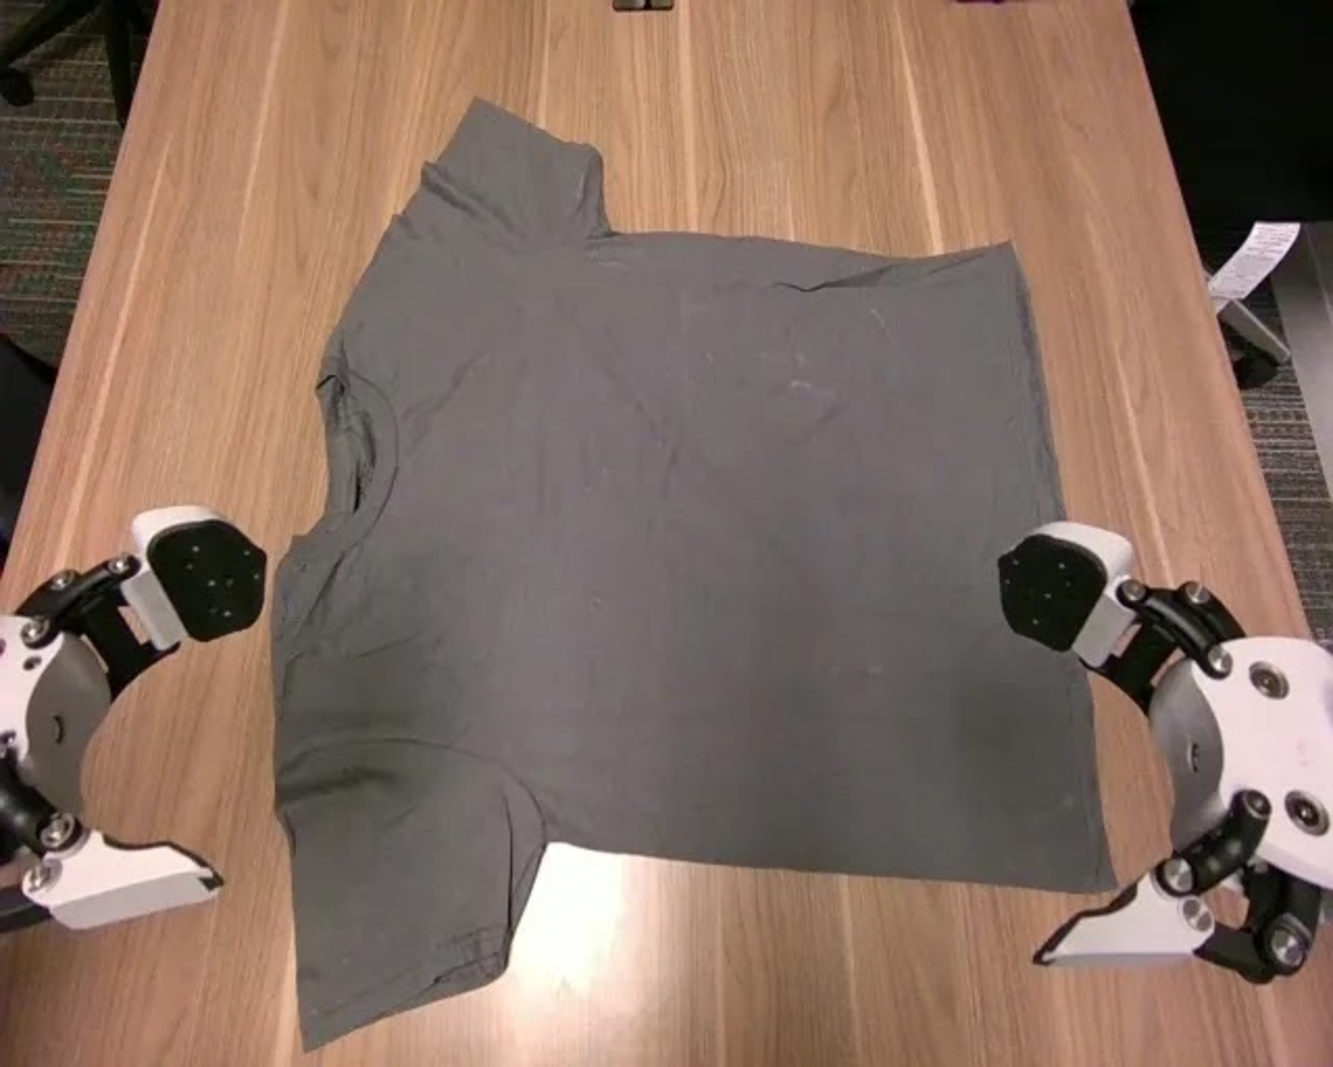
\includegraphics[width=3.2cm]{figures/agibot_seen/task2_r29_v1.pdf} & \centering\arraybackslash\scriptsize{Both arms fold the bottom of the gray short sleeve to the middle. They then pull the shirt toward the edge of the table. Next, both arms fold the top of the shirt down to the middle. Finally, the left arm grasps the collar and folds it down to finish.} \\
\cmidrule(lr){2-11}
\centering\textbf{\shortstack{Contact \\ Rich}} & 9 & \centering\textbf{Folding Shorts} & 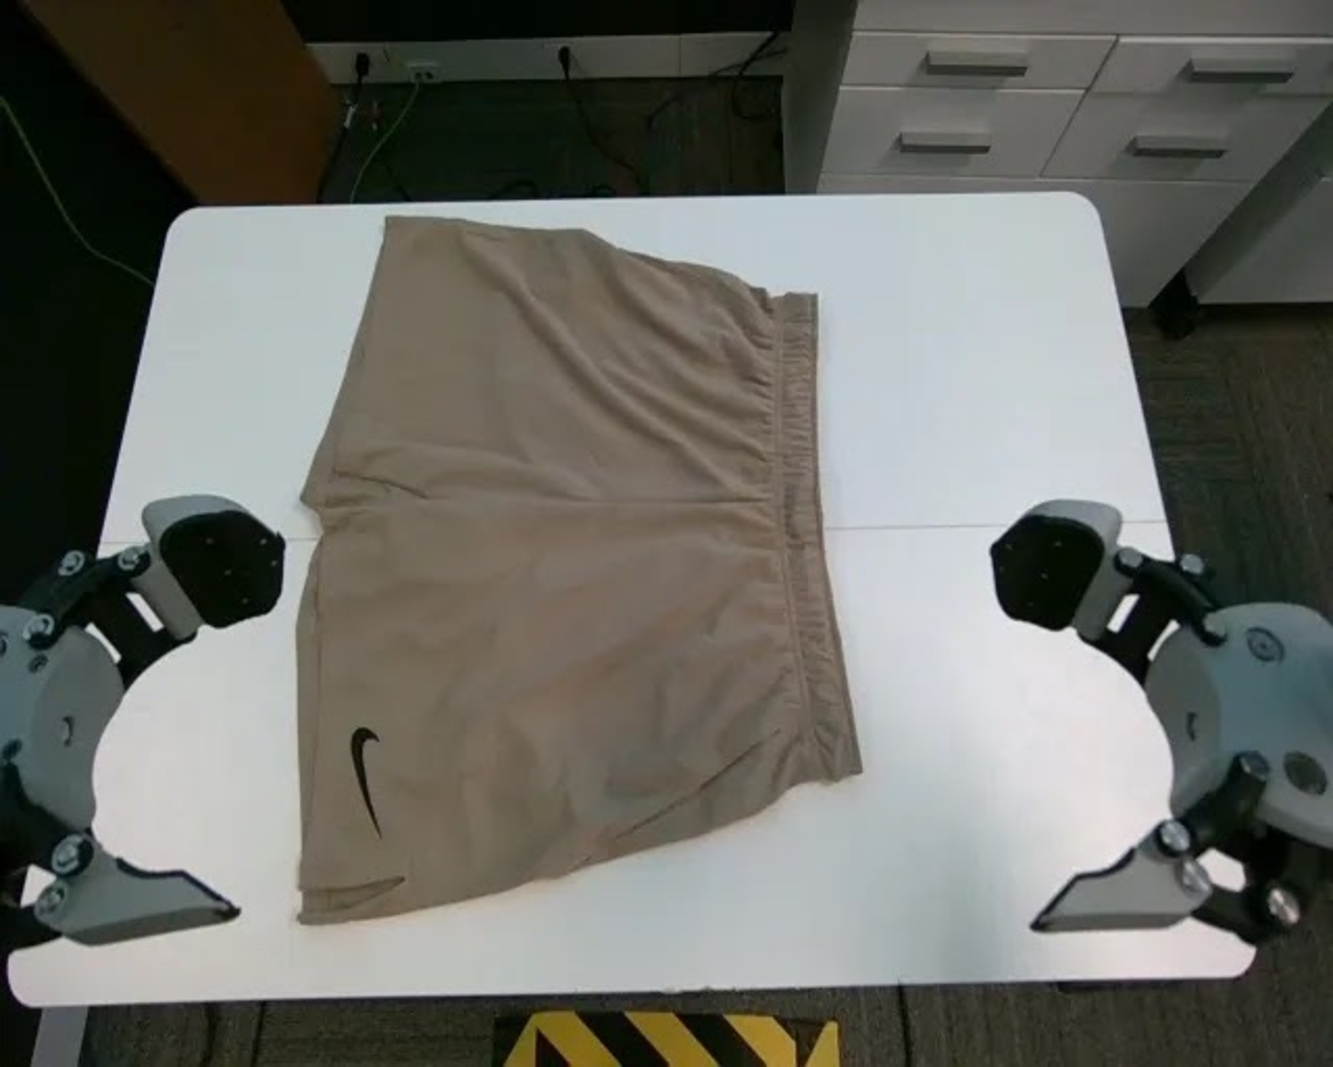
\includegraphics[width=3.2cm]{figures/agibot_seen/task3_r26_v1.pdf} & \centering\scriptsize{Both arms fold the bottom of the tan shorts toward the middle. Then, the right arm folds the shorts in half from right to left to complete the fold.} & 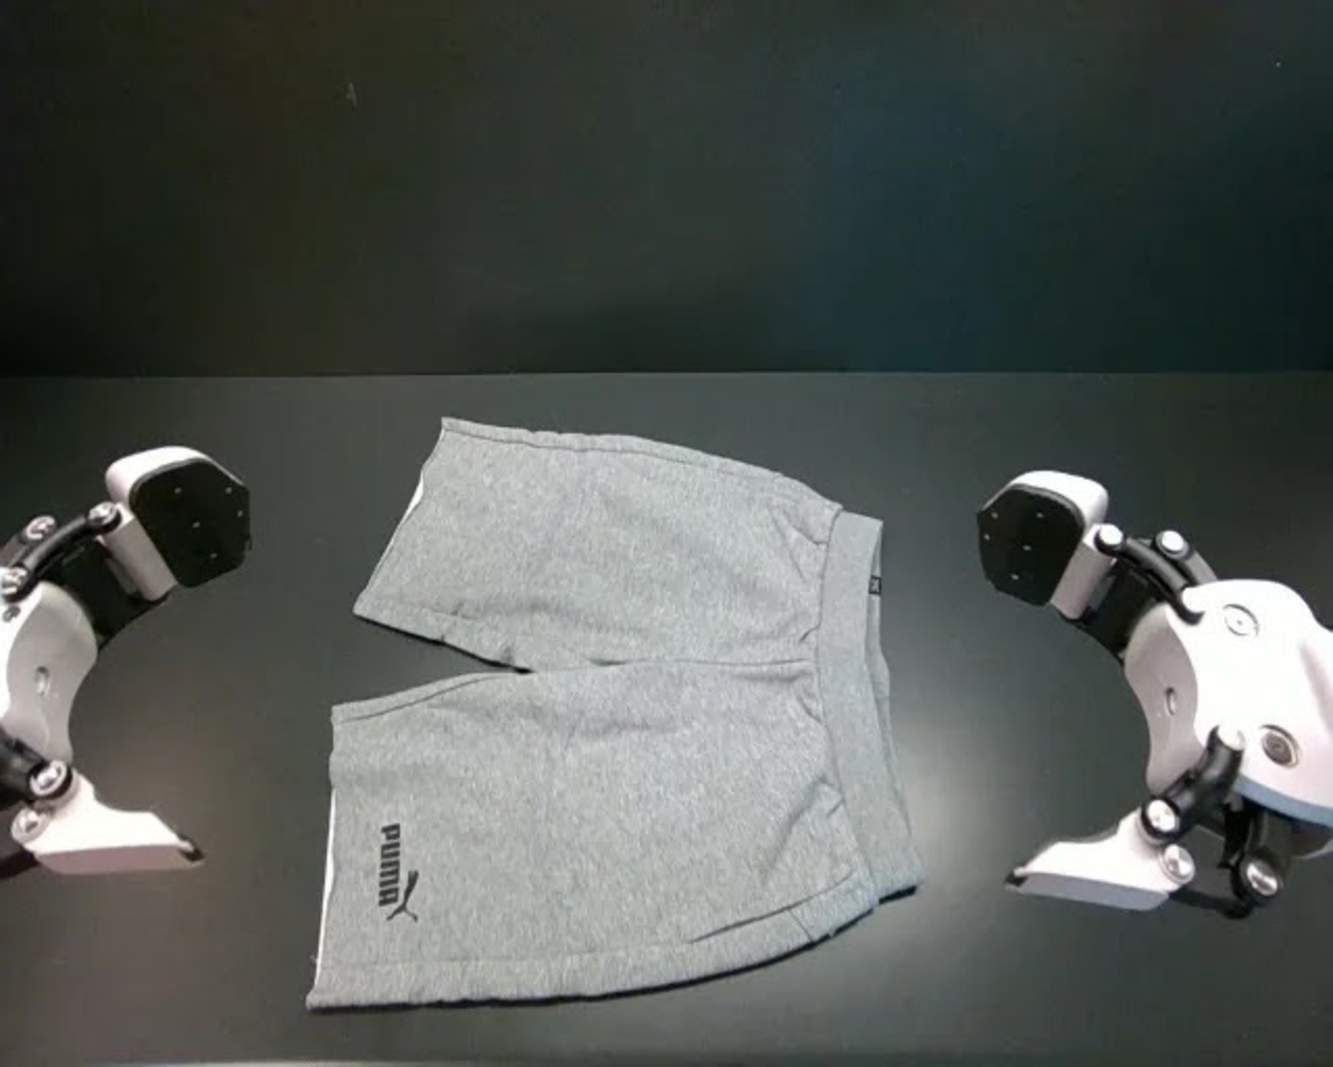
\includegraphics[width=3.2cm]{figures/agibot_seen/task3_r27_v1.pdf} & \centering\scriptsize{Both arms fold the bottom of the grey shorts toward the middle. Then, the right arm folds the shorts in half from right to left to complete the fold.} & 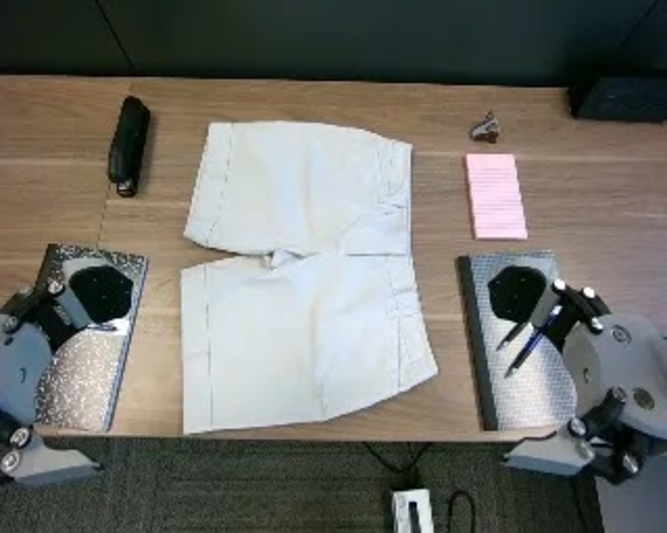
\includegraphics[width=3.2cm]{figures/agibot_seen/task3_r28_v1.pdf} & \centering\scriptsize{Both arms fold the bottom of the white shorts toward the middle. Then, the right arm folds the shorts in half from right to left to complete the task.} & 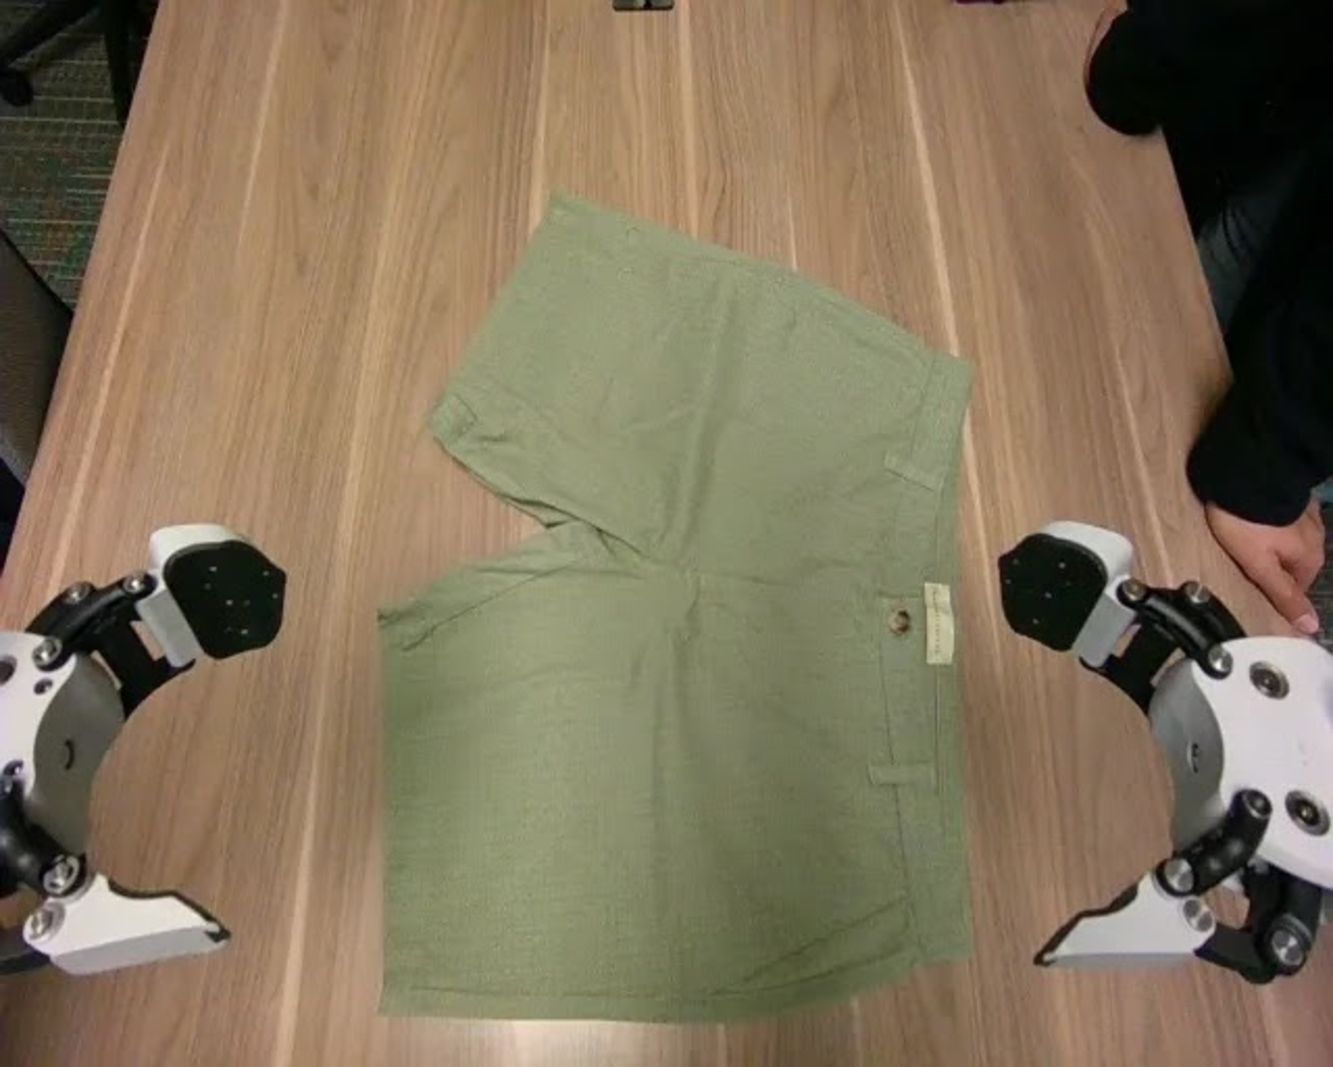
\includegraphics[width=3.2cm]{figures/agibot_seen/task3_r29_v1.pdf} & \centering\arraybackslash\scriptsize{Both arms fold the bottom of the green shorts toward the middle. Then, the right arm folds the shorts in half from right to left to complete the fold.} \\
\cmidrule(lr){2-11}
 & 10 & \centering\textbf{Stacking Clothes} & 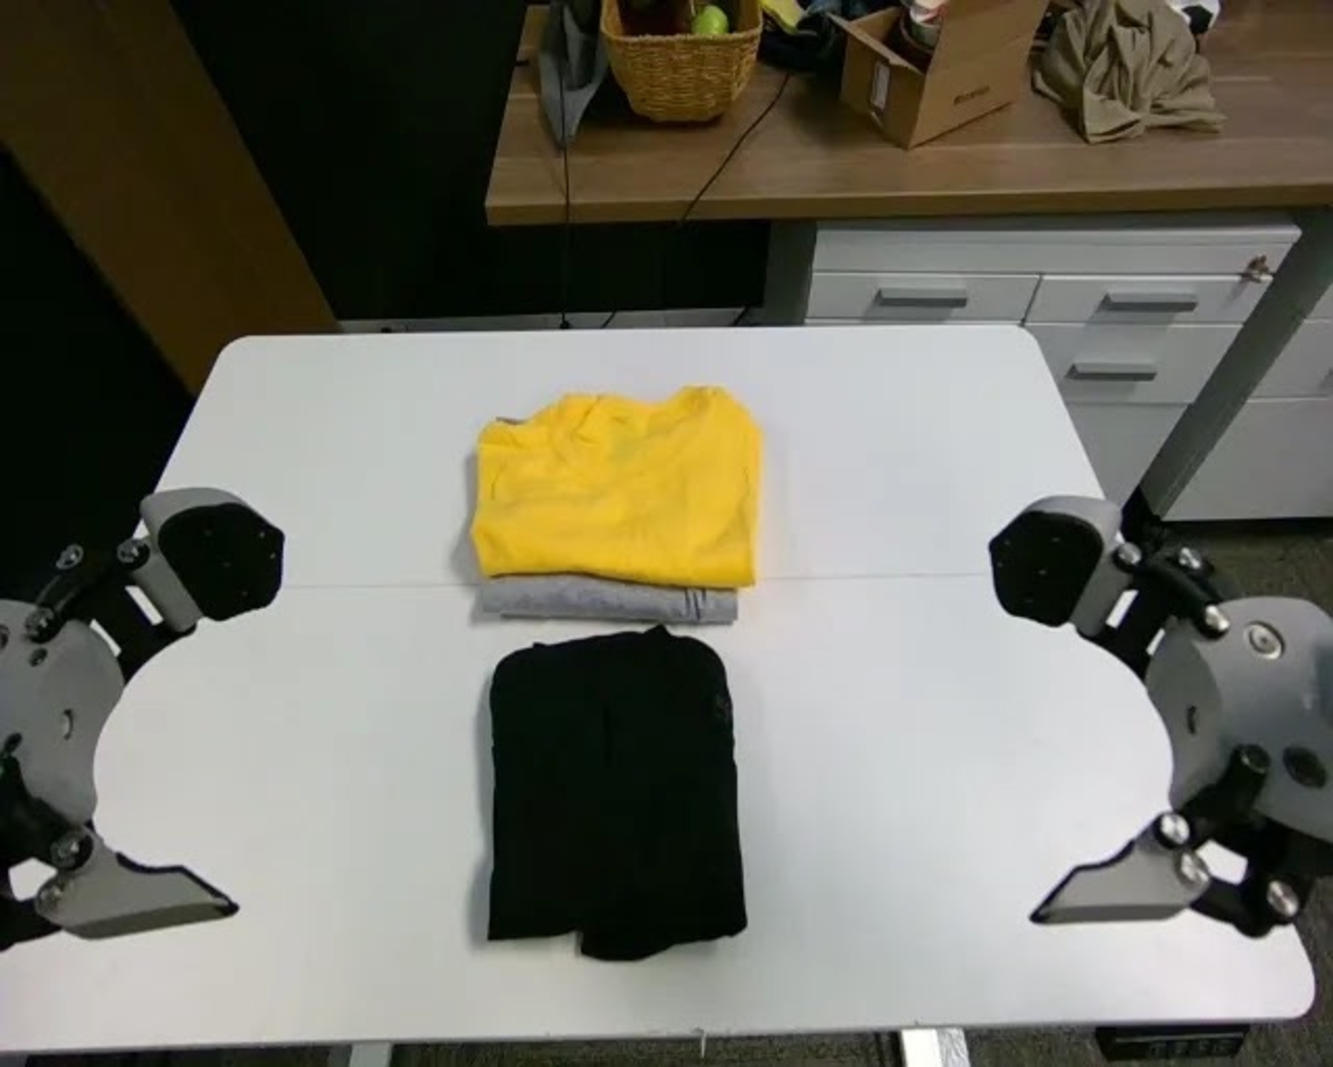
\includegraphics[width=3.2cm]{figures/agibot_seen/task4_r26_v1.pdf} & \centering\scriptsize{Both arms pick up the black shirt and place it on the stack of clothes.} & 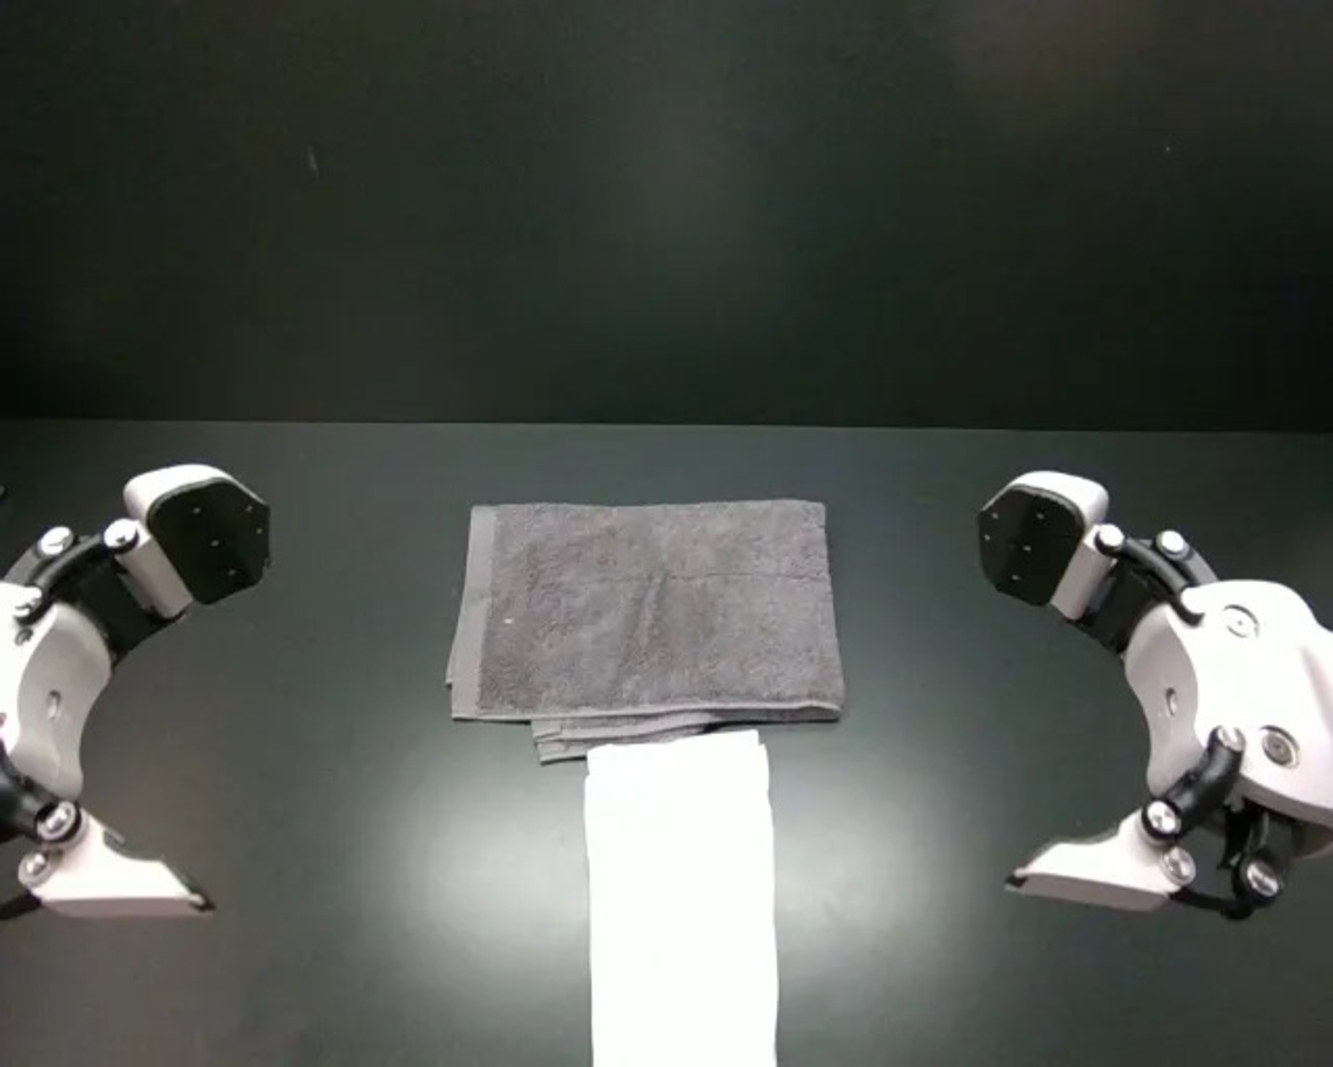
\includegraphics[width=3.2cm]{figures/agibot_seen/task4_r27_v1.pdf} & \centering\scriptsize{Both arms pick up the white shirt and place it on the gray towel.} & 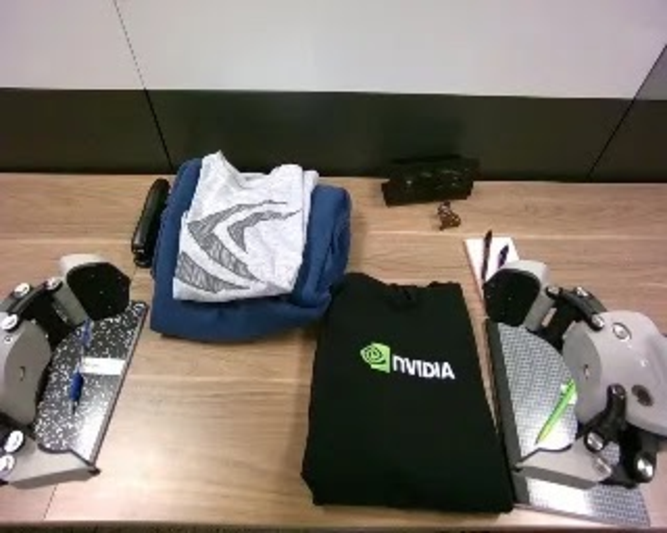
\includegraphics[width=3.2cm]{figures/agibot_seen/task4_r28_v1.pdf} & \centering\scriptsize{Both arms pick up the black hoodie and place it on the stack of clothes.} & 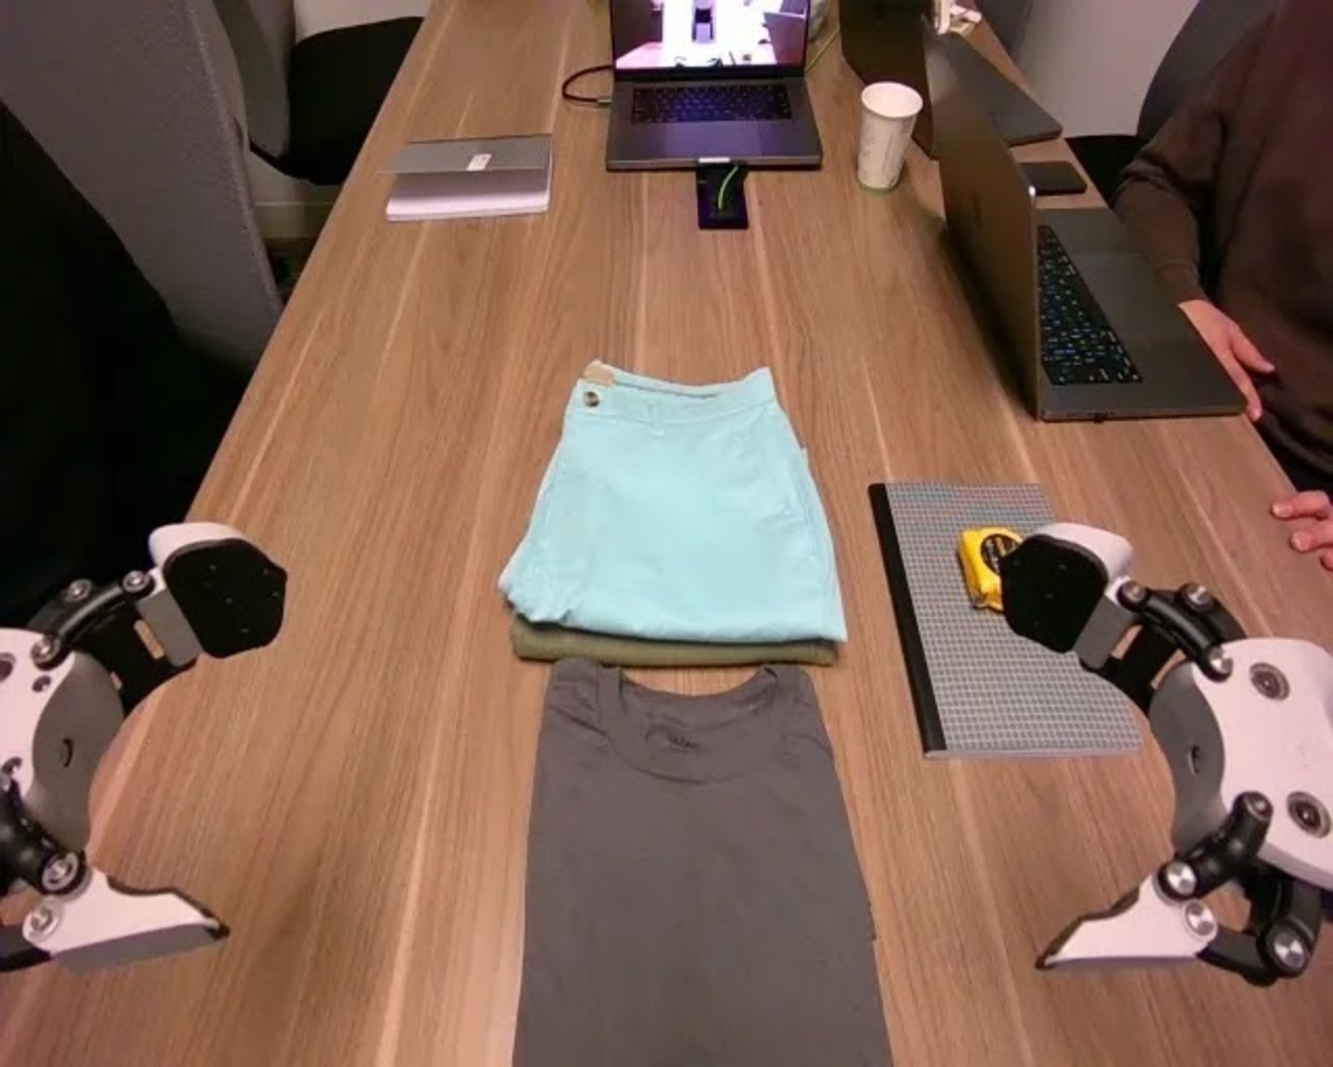
\includegraphics[width=3.2cm]{figures/agibot_seen/task4_r29_v1.pdf} & \centering\arraybackslash\scriptsize{Both arms pick up the dark gray shirt and place it on the stack of clothes.} \\
\bottomrule
\end{tabular}
}
\end{table*}






% \subsection{Unseen Tasks}
\begin{table*}[htbp]
\centering
\caption{\textbf{Unseen Tasks Evaluation Setup for AgiBot G1}}
\label{tab:unseen_tasks}
\setlength{\tabcolsep}{2pt}
\resizebox{\textwidth}{!}{
\begin{tabular}{cm{1.8cm}m{3.5cm}m{3.2cm}m{3.2cm}m{3.2cm}m{3.2cm}m{3.2cm}m{3.2cm}m{3.2cm}}
\toprule
\centering\textbf{\#} & \centering\textbf{Task} & \centering\textbf{Image} & \centering\textbf{Instruction} & \centering\textbf{Image} & \centering\textbf{Instruction} & \centering\textbf{Image} & \centering\textbf{Instruction} & \centering\textbf{Image} & \centering\arraybackslash\textbf{Instruction} \\
\midrule
1 & \centering\textbf{Untie Shoelaces} & 
\includegraphics[width=3.2cm]{figures/agibot_unseen/task1_r26_v1.pdf} & \centering\scriptsize{The robot coordinates both arms to simultaneously grasp the two loops of the shoelace. It then moves both arms outward in synchronized, opposing directions until the shoelace is fully untied.} & 
\includegraphics[width=3.2cm]{figures/agibot_unseen/task1_r27_v1.pdf} & \centering\scriptsize{The robot reaches its left arm to grasp the blue box and hold it steady. It then reaches its right arm toward the blue ribbon and moves it to untie the knot.} & 
\includegraphics[width=3.2cm]{figures/agibot_unseen/task1_r28_v1.pdf} & \centering\scriptsize{The robot coordinates both arms to simultaneously grasp the two loops of the knot of the box. It then moves both arms outward in synchronized, opposing directions until the knot of the box is fully untied.} & 
\includegraphics[width=3.2cm]{figures/agibot_unseen/task1_r29_v1.pdf} & \centering\arraybackslash\scriptsize{The robot coordinates both arms to simultaneously grasp the two loops of the knot of the package. It then moves both arms outward in synchronized, opposing directions until the knot of the package is fully untied.} \\
\midrule
2 & \centering\textbf{Remove\\/Put Hat} & 
\includegraphics[width=3.2cm]{figures/agibot_unseen/task2_r26_v1.pdf} & \centering\scriptsize{The robot reaches its right arm to gasp the crown and lifts it to remove it from the mannequin's head.} & 
\includegraphics[width=3.2cm]{figures/agibot_unseen/task2_r27_v1.pdf} & \centering\scriptsize{The robot reaches its left arm to grasp the hat and lifts it to remove it from the mannequin's head.} & 
\includegraphics[width=3.2cm]{figures/agibot_unseen/task2_r28_v1.pdf} & \centering\scriptsize{The robot reaches its left arm to grasp the hat and lifts it to remove it from the mannequin's head.} & 
\includegraphics[width=3.2cm]{figures/agibot_unseen/task2_r29_v1.pdf} & \centering\arraybackslash\scriptsize{The robot reaches its left arm to grasp the hat and lifts it to remove it from the mannequin's head.} \\
\midrule
3 & \centering\textbf{Draw Circle} & 
\includegraphics[width=3.2cm]{figures/agibot_unseen/task3_r26_v1.pdf} & \centering\scriptsize{The robot reaches its left arm to pick up the red marker and the left arm moves the marker to draw a circle on the book.} & 
\includegraphics[width=3.2cm]{figures/agibot_unseen/task3_r27_v1.pdf} & \centering\scriptsize{The robot reaches its right arm to pick up the marker and the right arm  draws a circle on the whiteboard with the marker.} & 
\includegraphics[width=3.2cm]{figures/agibot_unseen/task3_r28_v1.pdf} & \centering\scriptsize{The robot reaches its left arm to pick up the black marker and the left arm moves the marker to draw a circle on the paper} & 
\includegraphics[width=3.2cm]{figures/agibot_unseen/task3_r29_v1.pdf} & \centering\arraybackslash\scriptsize{The robot reaches its right arm to pick up the marker and the right arm moves the marker to draw a llne on the whiteboard.} \\
\midrule
4 & \centering\textbf{Take out Straw} & 
\includegraphics[width=3.2cm]{figures/agibot_unseen/task4_r26_v1.pdf} & \centering\scriptsize{The left arm holds the cup on the table. Then the right arm pulls the straw out of the cup.} & 
\includegraphics[width=3.2cm]{figures/agibot_unseen/task4_r27_v1.pdf} & \centering\scriptsize{The left arm holds the cup on the table. Then the right arm pulls the straw out of the cup.} & 
\includegraphics[width=3.2cm]{figures/agibot_unseen/task4_r28_v1.pdf} & \centering\scriptsize{The left arm holds the cup on the table. Then the right arm pulls the straw out of the cup.} & 
\includegraphics[width=3.2cm]{figures/agibot_unseen/task4_r29_v1.pdf} & \centering\arraybackslash\scriptsize{The right arm holds the cup on the table.Then the left arm pulls the straw out of the cup.} \\
\midrule
5 & \centering\textbf{Cube Stacking} & 
\includegraphics[width=3.2cm]{figures/agibot_unseen/task5_r26_v1.pdf} & \centering\scriptsize{The robot reaches its right arm to pick up the green cube, moves it over the red cube, and releases it to stack. It then reaches its right arm to pick up the yellow cube, moves it over the stack, and releases it onto the green cube to finish the task.} & 
\includegraphics[width=3.2cm]{figures/agibot_unseen/task5_r27_v1.pdf} & \centering\scriptsize{The robot reaches its right arm to pick up the red cube, moves it over the colorful cube, and releases it to stack. It then reaches its right arm to pick up the green cube, moves it over the red cube, and releases it to finish the tower.} & 
\includegraphics[width=3.2cm]{figures/agibot_unseen/task5_r28_v1.pdf} & \centering\scriptsize{The robot reaches its right arm to pick up the white cube, moves it over the green cube, and releases it to stack. It then reaches its left arm to pick up the blue cube, moves it over the stack, and releases it onto the white cube to finish the task.} & 
\includegraphics[width=3.2cm]{figures/agibot_unseen/task5_r29_v1.pdf} & \centering\arraybackslash\scriptsize{The robot reaches its right arm to pick up the red cube, moves it over the blue cube, and releases it to begin the stack. It then reaches its left arm to pick up the orange cube, moves it over the stack, and releases it onto the red cube to complete the three-tier structure.} \\
\midrule
6 & \centering\textbf{Painting} & 
\includegraphics[width=3.2cm]{figures/agibot_unseen/task6_r26_v1.pdf} & \centering\scriptsize{The left arm grabs the brush. Then left arm paints with the brush on the notebook} & 
\includegraphics[width=3.2cm]{figures/agibot_unseen/task6_r27_v1.pdf} & \centering\scriptsize{The right arm grabs the brush. Then right arm paints with the brush on the paper} & 
\includegraphics[width=3.2cm]{figures/agibot_unseen/task6_r28_v1.pdf} & \centering\scriptsize{The left arm grabs the brush. Then left arm paints with the brush on the notebook} & 
\includegraphics[width=3.2cm]{figures/agibot_unseen/task6_r29_v1.pdf} & \centering\arraybackslash\scriptsize{The right arm grabs the brush. Then right arm paints with the brush on the notebook} \\
\midrule
7 & \centering\textbf{Ironing} & 
\includegraphics[width=3.2cm]{figures/agibot_unseen/task7_r26_v1.pdf} & \centering\scriptsize{The robot reaches its left arm to grasp the iron and moves it across the shorts to iron it.} & 
\includegraphics[width=3.2cm]{figures/agibot_unseen/task7_r27_v1.pdf} & \centering\scriptsize{The robot reaches its right arm to grasp the iron and moves it across the shirt to iron it.} & 
\includegraphics[width=3.2cm]{figures/agibot_unseen/task7_r28_v1.pdf} & \centering\scriptsize{The robot reaches its left arm to grasp the iron and moves it across the shirt to iron it.} & 
\includegraphics[width=3.2cm]{figures/agibot_unseen/task7_r29_v1.pdf} & \centering\arraybackslash\scriptsize{The robot reaches its left arm to grasp the iron and moves it across the shirt to iron it.} \\
\midrule
8 & \centering\textbf{Shake Hands} & 
\includegraphics[width=3.2cm]{figures/agibot_unseen/task8_r26_v1.pdf} & \centering\scriptsize{The right arm of the robot grasp the human hand to shake hands. It then initiates a rhythmic up-and-down motion to perform the handshake.} & 
\includegraphics[width=3.2cm]{figures/agibot_unseen/task8_r27_v1.pdf} & \centering\scriptsize{The left arm shakes the hand of the human up and down} & 
\includegraphics[width=3.2cm]{figures/agibot_unseen/task8_r28_v1.pdf} & \centering\scriptsize{The right arm shakes the hand of the human up and down} & 
\includegraphics[width=3.2cm]{figures/agibot_unseen/task8_r29_v1.pdf} & \centering\arraybackslash\scriptsize{The left arm of the robot grasp the human hand to shake hands. It then initiates a rhythmic up-and-down motion to perform the handshake.} \\
\midrule
9 & \centering\textbf{Folding (Map)} & 
\includegraphics[width=3.2cm]{figures/agibot_unseen/task9_r26_v1.pdf} & \centering\scriptsize{The left arm grabs the left side of the map. The right arm folds the right side of the map. The left arm folds the left side of the map.} & 
\includegraphics[width=3.2cm]{figures/agibot_unseen/task9_r27_v1.pdf} & \centering\scriptsize{The left arm grabs the left side of the map. The right arm folds the right side of the map. The left arm folds the left side of the map.} & 
\includegraphics[width=3.2cm]{figures/agibot_unseen/task9_r28_v1.pdf} & \centering\scriptsize{The right arm grabs the right side of the map. The left arm folds the left side of the map. The right arm folds the right side of the map.} & 
\includegraphics[width=3.2cm]{figures/agibot_unseen/task9_r29_v1.pdf} & \centering\arraybackslash\scriptsize{The right arm grabs the right side of the map.The left arm folds the left side of the map. The right arm folds the right side of the map.} \\
\midrule
10 & \centering\textbf{Pulling Cart} & 
\includegraphics[width=3.2cm]{figures/agibot_unseen/task10_r26_v1.pdf} & \centering\scriptsize{The robot reaches its right arm to grasp the cart and pulls it.} & 
\includegraphics[width=3.2cm]{figures/agibot_unseen/task10_r27_v1.pdf} & \centering\scriptsize{The robot reaches its left arm to grasp the cart and pulls it.} & 
\includegraphics[width=3.2cm]{figures/agibot_unseen/task10_r28_v1.pdf} & \centering\scriptsize{The robot reaches its right arm to grasp the cart and pulls it.} & 
\includegraphics[width=3.2cm]{figures/agibot_unseen/task10_r29_v1.pdf} & \centering\arraybackslash\scriptsize{The robot reaches its left arm to grasp the cart and pulls it forward.} \\
\bottomrule
\end{tabular}
}
\end{table*}
